\documentclass[14pt]{extarticle}

\usepackage[table]{xcolor} % colored lines for tables
\usepackage[normalem]{ulem} % strike through text
\usepackage{amsmath,mathtools,amsfonts,amsthm,amssymb,hyperref}
\usepackage{parskip,geometry,latexsym,bookmark,mathtools,float,cancel}
\usepackage{tcolorbox,bm}

\newtheorem{defn}{Definition}
\newtheorem{thm}{Theorem}
\newtheorem{claim}{Claim}
\newtheorem{lemma}{Lemma}

\newcommand{\dps}{\displaystyle}
\newcommand{\es}{\varnothing}
\newcommand{\fbl}{\underline{\hspace{1cm}}\,\,}
\newcommand{\R}{\mathbb{R}}
\newcommand{\Q}{\mathbb{Q}}
\newcommand{\Z}{\mathbb{Z}}
\newcommand{\from}{\leftarrow}
\newcommand{\true}{{\bf t}}
\newcommand{\false}{{\bf c}}
\newcommand{\bic}{\leftrightarrow}
\newcommand{\da}{\downarrow}
\newcommand{\fa}{\forall}
\newcommand{\te}{\exists}
\newcommand{\cy}{\color{cyan}}

\newcommand{\colsq}[1]{{\color{#1} $\blacksquare$}}

\newcommand{\base}[1]{{\cy #1}} % for log bases
\newcommand{\floor}[1]{{\left\lfloor#1\right\rfloor}}
\newcommand{\ceil}[1]{{\left\lceil#1\right\rceil}}
\newcommand\Ccancel[2][black]{\renewcommand\CancelColor{\color{#1}}\cancel{#2}}
\newcommand\Cbcancel[2][black]{\renewcommand\CancelColor{\color{#1}}\bcancel{#2}}
\newcommand\Cyancel[2][cyan]{\renewcommand\CancelColor{\color{#1}}\cancel{#2}}

%\renewcommand{\arraystretch}{1.2}
%\setlength{\extrarowheight}{10pt}

\hypersetup{colorlinks,allcolors=blue,linktoc=all}
\geometry{a4paper}
\geometry{margin=0.42in}

\title{Solutions to Chapter 10, Susanna Epp Discrete Math 5th Edition}

\author{https://github.com/spamegg1}

\begin{document}
\maketitle
\tableofcontents


\section{Exercise Set 10.1}
\subsection{Exercise 1}
In the graph below, determine whether the following walks are trails, paths, closed walks, circuits, simple circuits, or 
just walks.

\begin{figure}[ht!]
\centering
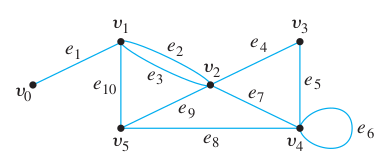
\includegraphics[scale=0.6]{../images/10.1.1.png}
\end{figure}

\subsubsection{(a)}
\(v_0e_1v_1e_{10}v_5e_9v_2e_2v_1\)

\begin{proof}
trail (no repeated edge), not a path (has a repeated vertex, \(v_1\)), not a circuit

\end{proof}

\subsubsection{(b)}
\(v_4e_7v_2e_9v_5e_{10}v_1e_3v_2e_9v_5\)
\begin{proof}
walk, not a trail (has a repeated edge, \(e_9\)), not a circuit
\end{proof}

\subsubsection{(c)}
\(v_2\)
\begin{proof}
closed walk (starts and ends at the same vertex), trail (no repeated edge since no edge), not a path or a circuit (since 
no edge)
\end{proof}

\subsubsection{(d)}
\(v_5v_2v_3v_4v_4v_5\)
\begin{proof}
circuit, not a simple circuit (repeated vertex, \(v_4\))
\end{proof}

\subsubsection{(e)}
\(v_2v_3v_4v_5v_2v_4v_3v_2\)
\begin{proof}
closed walk (starts and ends at the same vertex but has repeated edges, \(\{v_2, v_3\}\) and \(\{v_3, v_4\}\))
\end{proof}

\subsubsection{(f)}
\(e_5e_8e_{10}e_3\)
\begin{proof}
path
\end{proof}

\subsection{Exercise 2}
\begin{figure}[ht!]
\centering
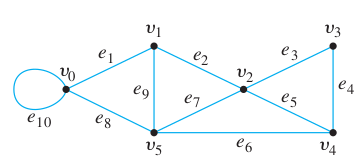
\includegraphics[scale=0.7]{../images/10.1.2.png}
\end{figure}

In the graph, determine whether the following walks are trails, paths, closed walks, circuits, simple circuits, or 
just walks.

\subsubsection{(a)}
\(v_1e_2v_2e_3v_3e_4v_4e_5v_2e_2v_1e_1v_0\)

\begin{proof}
walk (not closed), not a trail or circuit (has repeated edge \(e_2\)), not a path (has repeated vertex \(v_2\)), 
\end{proof}

\subsubsection{(b)}
\(v_2v_3v_4v_5v_2\)
\begin{proof}
simple circuit (only has the first + last vertex repeated, no repeated edge)
\end{proof}

\subsubsection{(c)}
\(v_4v_2v_3v_4v_5v_2v_4\)
\begin{proof}
closed walk, not a trail, path, circuit (has repeated edge \(e_5\) and vertex \(v_2\))
\end{proof}

\subsubsection{(d)}
\(v_2v_1v_5v_2v_3v_4v_2\)
\begin{proof}
circuit, not simple circuit (has non-first, non-last vertex repeated: \(v_2\))
\end{proof}

\subsubsection{(e)}
\(v_0v_5v_2v_3v_4v_2v_1\)
\begin{proof}
trail (no repeated edge), not a path (repeated vertex \(v_2\)), not a closed walk or circuit 
\end{proof}

\subsubsection{(f)}
\(v_5v_4v_2v_1\)

\begin{proof}
path (no repeated vertex), not a closed walk or circuit
\end{proof}

\subsection{Exercise 3}
Let \(G\) be the graph 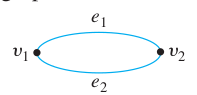
\includegraphics[scale=0.6]{../images/10.1.3.png} and consider the walk \(v_1e_1v_2e_2v_1\).

\subsubsection{(a)}
Can this walk be written unambiguously as \(v_1v_2v_1\)? Why?
\begin{proof}
No, because \(v_1v_2v_1\) could also refer to \(v_1e_2v_2e_1v_1\).
\end{proof}

\subsubsection{(b)}
Can this walk be written unambiguously as \(e_1e_2\)? Why?
\begin{proof}
Yes.
\end{proof}

\subsection{Exercise 4}
Consider the following graph:
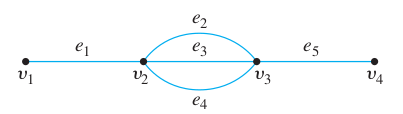
\includegraphics[scale=0.5]{../images/10.1.4.png}

\subsubsection{(a)}
How many paths are there from \(v_1\) to \(v_4\)?
\begin{proof}
3: \(e_1e_2e_5, e_1e_3e_5, e_1e_4e_5\).
\end{proof}

\subsubsection{(b)}
How many trails are there from \(v_1\) to \(v_4\)?
\begin{proof}
3! + 3 = 9 (The three paths from part (a) are also trails, and there are an additional 3! trails with vertices \(v_1, v_2, 
v_3, v_2, v_3, v_4\). The reason is that from \(v_2\) there are 3 choices of an edge to go to \(v_3\), then 2 choices of a 
different edge to go back to \(v_2\), and then 1 choice of a different edge to return to \(v_3\).
\end{proof}

\subsubsection{(c)}
How many walks are there from \(v_1\) to \(v_4\)?
\begin{proof}
Infinitely many. (Since a walk may have repeated edges, a walk from \(v_1\) to \(v_4\) may contain an arbitrarily large 
number of repetitions of edges joining a pair of vertices along the way.)
\end{proof}

\subsection{Exercise 5}
Consider the following graph:
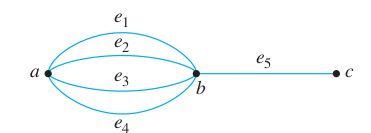
\includegraphics[scale=0.5]{../images/10.1.5.png}

\subsubsection{(a)}
How many paths are there from \(a\) to \(c\)?
\begin{proof}
4: \(e_1e_5, e_2e_5, e_3e_5, e_4e_5\).
\end{proof}

\subsubsection{(b)}
How many trails are there from \(a\) to \(c\)?
\begin{proof}
4! + 4 = 28 (The 4 paths from part (a) are also trails, and there are an additional 4! trails with vertices \(a,b,a,b,c\). 
The reason is that from \(a\) there are 4 choices of an edge to go to \(b\), then 3 choices of a different edge to go back 
to \(a\), then 2 choices of a different edge to go back to \(b\), and then 1 choice of a different edge to go to \(c\).
\end{proof}

\subsubsection{(c)}
How many walks are there from \(a\) to \(c\)?
\begin{proof}
Infinitely many. (Since a walk may have repeated edges, a walk from \(a\) to \(c\) may contain an arbitrarily large number of 
repetitions of edges joining a pair of vertices along the way.)
\end{proof}

\subsection{Exercise 6}
An edge whose removal disconnects the graph of which it is a part is called a bridge. Find all bridges for each of the 
graphs at the top of the next page.

\subsubsection{(a)}
\begin{figure}[ht!]
\centering
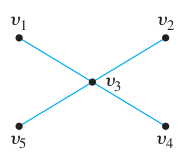
\includegraphics[scale=0.6]{../images/10.1.6.a.png}
\end{figure}

\begin{proof}
\(\{v_1, v_3\}, \{v_2, v_3\}, \{v_4, v_3\}\), and \(\{v_5, v_3\}\) are all the bridges.
\end{proof}

\subsubsection{(b)}
\begin{figure}[ht!]
\centering
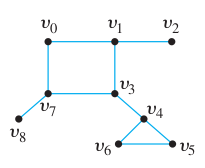
\includegraphics[scale=0.6]{../images/10.1.6.b.png}
\end{figure}

\begin{proof}
\(\{v_1, v_2\}, \{v_3, v_4\}, \{v_7, v_8\}\) are all the bridges.
\end{proof}

\subsubsection{(c)}
\begin{figure}[ht!]
\centering
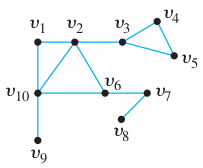
\includegraphics[scale=0.6]{../images/10.1.6.c.png}
\end{figure}

\begin{proof}
\(\{v_2, v_3\}, \{v_6, v_7\}, \{v_7, v_8\}, \{v_9, v_{10}\}\) are all the bridges. (see below)
\end{proof}

\subsection{Exercise 7}
Given any positive integer \(n\), (a) find a connected graph with \(n\) edges such that removal of just one edge 
disconnects the graph; (b) find a connected graph with \(n\) edges that cannot be disconnected by the removal of any 
single edge.

\begin{proof}
(a) Consider a line graph with \(n\) edges and \(n+1\) vertices that looks like: \\\(\cdot-\cdot-\ldots-\cdot-\cdot\) 
: \(v_1e_1v_2e_2 \ldots v_ne_nv_{n+1}\). Then removing any one edge will break the line and disconnect the graph.

(b) Consider a closed loop graph with \(n\) edges and \(n\) vertices: \(v_1e_1v_2e_2 \ldots v_ne_nv_1\) 

\begin{figure}[ht!]
\centering
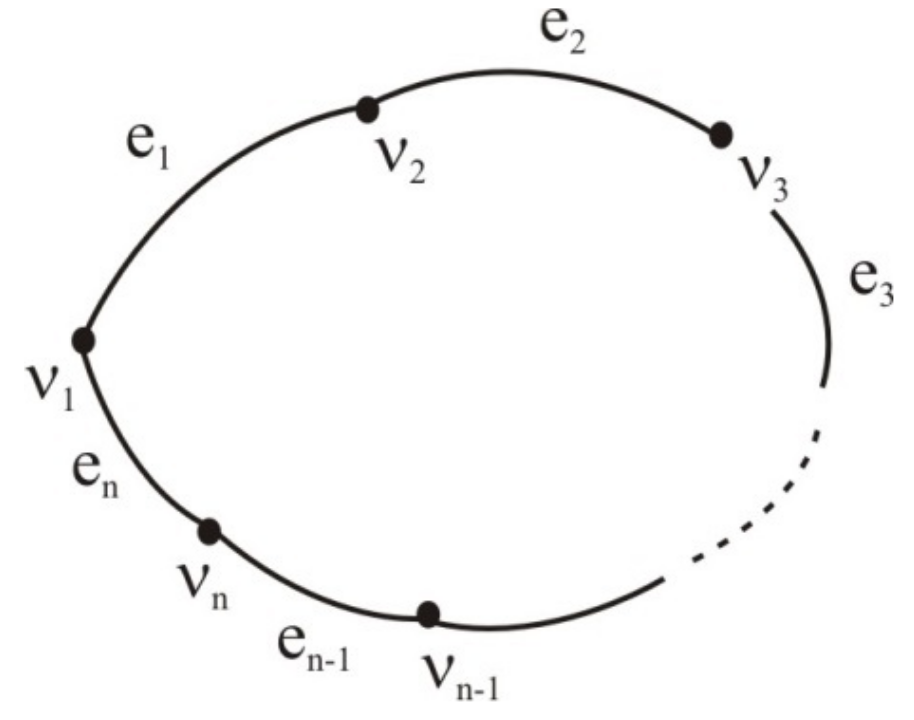
\includegraphics[scale=0.2]{../images/10.1.7.png}
\end{figure}

(so the last edge \(e_n\) connects back to the first vertex \(v_1\), closing the loop). Then removing any one edge will 
break the loop, but it will remain connected.
\end{proof}

\subsection{Exercise 8}
Find the number of connected components for each of the following graphs.

\subsubsection{(a)}
\begin{figure}[ht!]
\centering
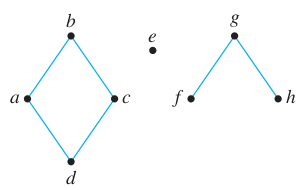
\includegraphics[scale=0.6]{../images/10.1.8.a.1.png}
\end{figure}

\begin{proof}
Three connected components, as shown in the next column.

\begin{figure}[ht!]
\centering
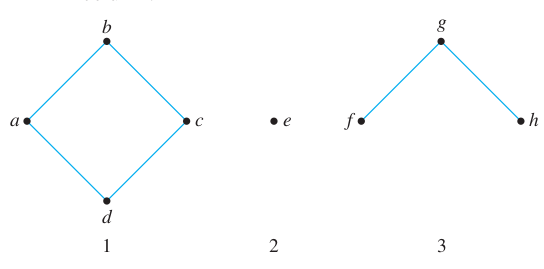
\includegraphics[scale=0.5]{../images/10.1.8.a.2.png}
\end{figure}
\end{proof}

\subsubsection{(b)}
\begin{figure}[ht!]
\centering
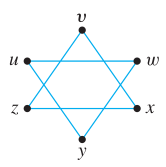
\includegraphics[scale=0.5]{../images/10.1.8.b.1.png}
\end{figure}

\begin{proof}
Two connected components: the two ``triangles'' \(v-x-z\) and \(u-w-y\).
\end{proof}

\subsubsection{(c)}
\begin{figure}[ht!]
\centering
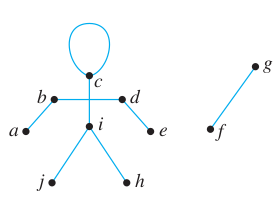
\includegraphics[scale=0.6]{../images/10.1.8.c.1.png}
\end{figure}

\begin{proof}
Three connected components: the ``arms and shoulders'' part \(a-b-d-e\), the ``head-torso-legs'' part \(c-i-j-h\) and the
part \(f-g\).
\end{proof}

\subsubsection{(d)}
\begin{figure}[ht!]
\centering
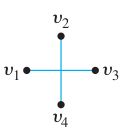
\includegraphics[scale=0.5]{../images/10.1.8.d.1.png}
\end{figure}

\begin{proof}
Two connected components: \(v_1-v_3\) and \(v_2-v_4\).
\end{proof}

\subsection{Exercise 9}
Each of (a)–(c) describes a graph. In each case answer yes, no, or not necessarily to this question: Does the graph have 
an Euler circuit? Justify your answers.

\subsubsection{(a)}
\(G\) is a connected graph with five vertices of degrees 2, 2, 3, 3, and 4.
\begin{proof}
No. This graph has two vertices of odd degree, whereas all vertices of a graph with an Euler circuit have even degree.
\end{proof}

\subsubsection{(b)}
\(G\) is a connected graph with five vertices of degrees 2, 2, 4, 4, and 6.
\begin{proof}
Yes (connected, all vertices have even degree, so by Theorem 10.1.4).
\end{proof}

\subsubsection{(c)}
\(G\) is a graph with five vertices of degrees 2, 2, 4, 4, and 6.
\begin{proof}
Not necessarily (if \(G\) is connected then yes by Theorem 10.1.4).
\end{proof}

\subsection{Exercise 10}
The solution for Example 10.1.6 shows a graph for which every vertex has even degree but which does not have an Euler 
circuit. Give another example of a graph satisfying these conditions.

\begin{proof}
Just take two disconnected squares: graphs with 4 vertices each. Considered together as one graph, each vertex has degree
2 but there is no Euler circuit.
\end{proof}

\subsection{Exercise 11}
Is it possible for a citizen of Königsberg to make a tour of the city and cross each bridge exactly twice? (See figure 
below.) Explain.

\begin{figure}[ht!]
\centering
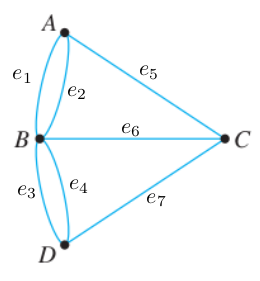
\includegraphics[scale=0.5]{../images/10.1.11.png}
\end{figure}

\begin{proof}
\(Ae_1Be_2Ae_5Ce_6Be_3De_4Be_6Ce_7De_3Be_4De_7Ce_5Ae_1Be_2A\). 
\end{proof}

{\bf \cy Determine which of the graphs in 12–17 have Euler circuits. If the graph does not have an Euler circuit, explain 
why not. If it does have an Euler circuit, describe one.}

\subsection{Exercise 12}
\begin{figure}[ht!]
\centering
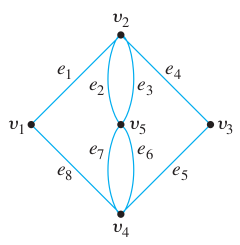
\includegraphics[scale=0.4]{../images/10.1.12.png}
\end{figure}

\begin{proof}
One Euler circuit is \(e_4e_5e_6e_3e_2e_7e_8e_1\).
\end{proof}

\subsection{Exercise 13}
\begin{figure}[ht!]
\centering
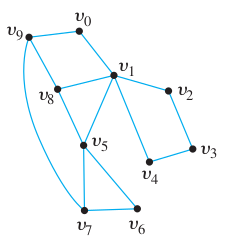
\includegraphics[scale=0.5]{../images/10.1.13.png}
\end{figure}

\begin{proof}
No Euler circuit, since \(v_1\) has odd degree (5).
\end{proof}

\subsection{Exercise 14}
\begin{figure}[ht!]
\centering
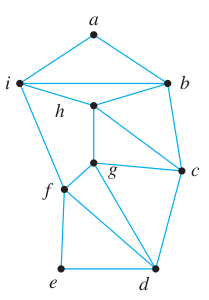
\includegraphics[scale=0.4]{../images/10.1.14.png}
\end{figure}

\begin{proof}
One Euler circuit is \(iabihbchgcdgfdefi\).
\end{proof}

\subsection{Exercise 15}
\begin{figure}[ht!]
\centering
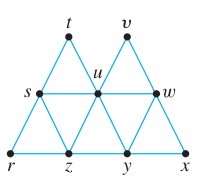
\includegraphics[scale=0.5]{../images/10.1.15.png}
\end{figure}

\begin{proof}
One Euler circuit is \(rzyxwyuzsuwvutsr\).
\end{proof}

\subsection{Exercise 16}
\begin{figure}[ht!]
\centering
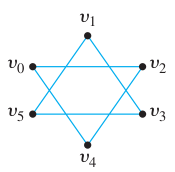
\includegraphics[scale=0.6]{../images/10.1.16.png}
\end{figure}

\begin{proof}
No Euler circuit (graph is not connected).
\end{proof}

\subsection{Exercise 17}
\begin{figure}[ht!]
\centering
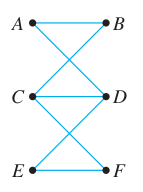
\includegraphics[scale=0.6]{../images/10.1.17.png}
\end{figure}

\begin{proof}
No Euler circuit (C has odd degree 3).
\end{proof}

\subsection{Exercise 18}
\begin{figure}[ht!]
\centering
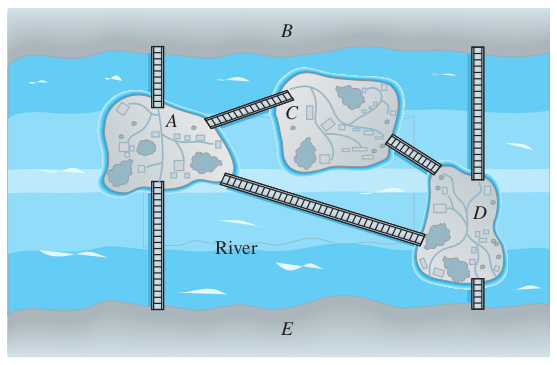
\includegraphics[scale=0.5]{../images/10.1.18.png}
\end{figure}

Is it possible to take a walk around the city whose map is shown above, starting and ending at the same point and 
crossing each bridge exactly once? If so, how can this be done?

\begin{proof}
DCADBAED
\end{proof}

{\bf \cy For each of the graphs in \(19-21\), determine whether there is an Euler trial from \(u\) to \(w\). If there 
is, find such a trail.}

\subsection{Exercise 19}
\begin{figure}[ht!]
\centering
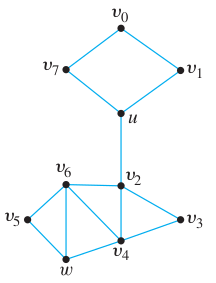
\includegraphics[scale=0.4]{../images/10.1.19.png}
\end{figure}

\begin{proof}
There is an Euler trail since deg(\(u\)) and deg(\(w\)) are odd, all other vertices have positive even degree, and the 
graph is connected. \(uv_1v_0v_7uv_2v_3v_4v_2v_6v_4wv_5v_6w\) is one Euler trail.
\end{proof}

\subsection{Exercise 20}
\begin{figure}[ht!]
\centering
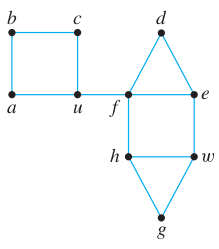
\includegraphics[scale=0.5]{../images/10.1.20.png}
\end{figure}

\begin{proof}
No Euler trail, since there are 4 vertices with odd degrees: \(u, e, h, w\).
\end{proof}

\subsection{Exercise 21}
\begin{figure}[ht!]
\centering
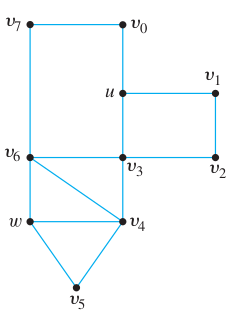
\includegraphics[scale=0.5]{../images/10.1.21.png}
\end{figure}

\begin{proof}
One Euler trail is \(uv_0v_7v_6v_3uv_1v_2v_3v_4v_6wv_4v_5w\).
\end{proof}

\subsection{Exercise 22}
\begin{figure}[ht!]
\centering
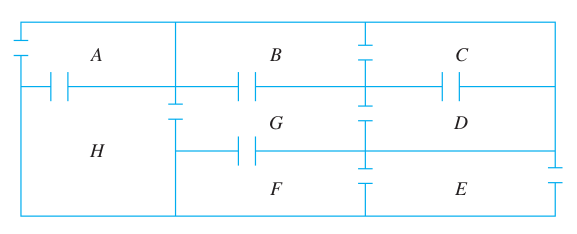
\includegraphics[scale=0.4]{../images/10.1.22.png}
\end{figure}

The following is a floor plan of a house. Is it possible to enter the house in room A, travel through every interior 
doorway of the house exactly once, and exit out of room E? If so, how can this be done?

\begin{proof}
Let rooms be vertices, let the outside also be a vertex (I). Then

\begin{figure}[ht!]
\centering
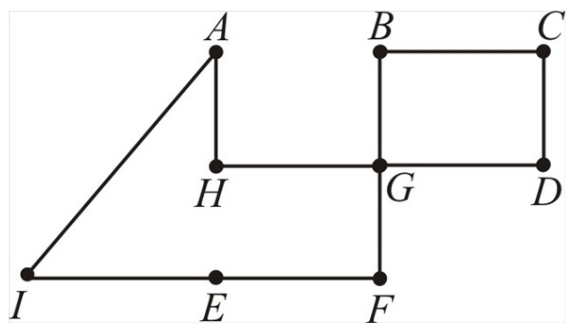
\includegraphics[scale=0.25]{../images/10.1.22.b.png}
\end{figure}

One Euler circuit is: IAHGBCDGFEI
\end{proof}

\subsection{Exercise 23}
Find all subgraphs of each of the following graphs.

\subsubsection{(a)}
\begin{figure}[ht!]
\centering
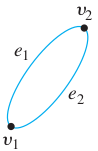
\includegraphics[scale=0.5]{../images/10.1.23.a.1.png}
\end{figure}

\begin{proof}
The nonempty subgraphs are as follows:

\begin{figure}[ht!]
\centering
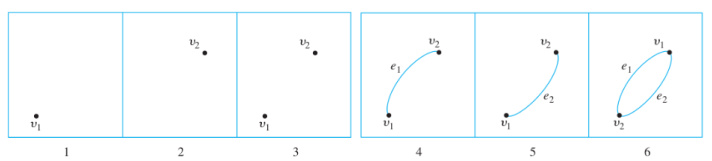
\includegraphics[scale=0.6]{../images/10.1.23.a.2.png}
\end{figure}
\end{proof}

\subsubsection{(b)}
\begin{figure}[ht!]
\centering
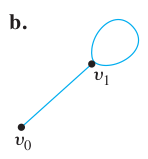
\includegraphics[scale=0.5]{../images/10.1.23.b.1.png}
\end{figure}

\begin{proof}
The nonempty subgraphs are as above.

\begin{figure}[ht!]
\centering
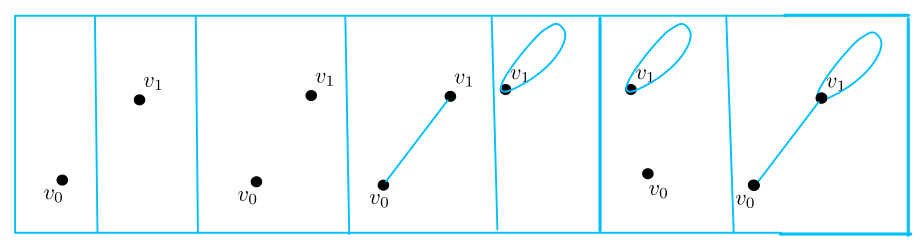
\includegraphics[scale=0.3]{../images/10.1.23.b.2.png}
\end{figure}
\end{proof}

\subsubsection{(c)}
\begin{figure}[ht!]
\centering
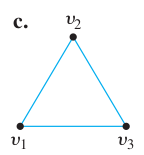
\includegraphics[scale=0.5]{../images/10.1.23.c.1.png}
\end{figure}

\begin{proof}
The nonempty subgraphs are as follows:

\begin{figure}[ht!]
\centering
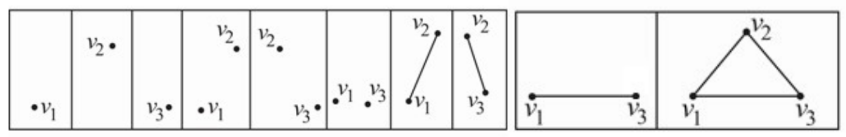
\includegraphics[scale=0.5]{../images/10.1.23.c.2.png}
\end{figure}
\end{proof}

\begin{tcolorbox}[colframe=cyan]
{\bf \cy Definition:} If \(G\) is a simple graph, the complement of \(G\), denoted \(G'\), is obtained as follows: 
The vertex set of \(G'\) is identical to the vertex set of \(G\). However, two distinct vertices \(v\) and \(w\) of \(G'\) 
are connected by an edge if, and only if, \(v\) and \(w\) are not connected by an edge in \(G\). 

For example, if \(G\) is the graph 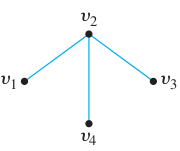
\includegraphics[scale=0.4]{../images/10.1.24.1.png} then \(G'\) is the graph 
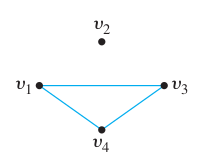
\includegraphics[scale=0.4]{../images/10.1.24.2.png}.
\end{tcolorbox}

\subsection{Exercise 24}
Find the complement of each of the following graphs.

\subsubsection{(a)}
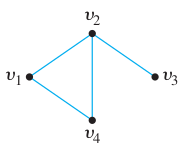
\includegraphics[scale=0.5]{../images/10.1.24.a.1.png}
{\it Proof.}
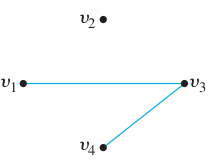
\includegraphics[scale=0.5]{../images/10.1.24.a.2.png}

\subsubsection{(b)}
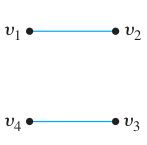
\includegraphics[scale=0.5]{../images/10.1.24.b.1.png}
{\it Proof.}
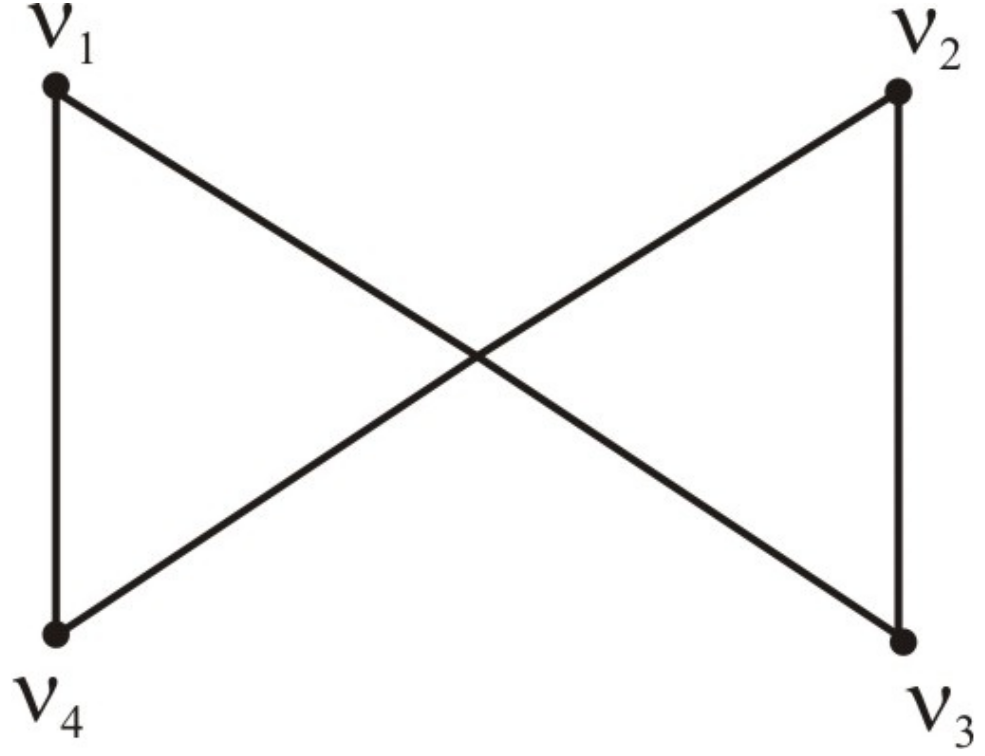
\includegraphics[scale=0.1]{../images/10.1.24.b.2.png}

\subsection{Exercise 25}
\subsubsection{(a)}
Find the complement of the graph \(K_4\), the complete graph on four vertices.

\begin{proof}
This is the graph with four vertices and no edges.
\end{proof}

\subsubsection{(b)}
Find the complement of the graph \(K_{3,2}\), the complete bipartite graph on (3, 2) vertices.

\begin{proof}
This is the union of separate graphs \(K_3\) (a triangle) and \(K_2\) (a line).
\end{proof}

\subsection{Exercise 26}
Suppose that in a group of five people A, B, C, D, and E the following pairs of people are acquainted with each other. A 
and C, A and D, B and C, C and D, C and E.

\subsubsection{(a)}
Draw a graph to represent this situation.

{\it Proof.}
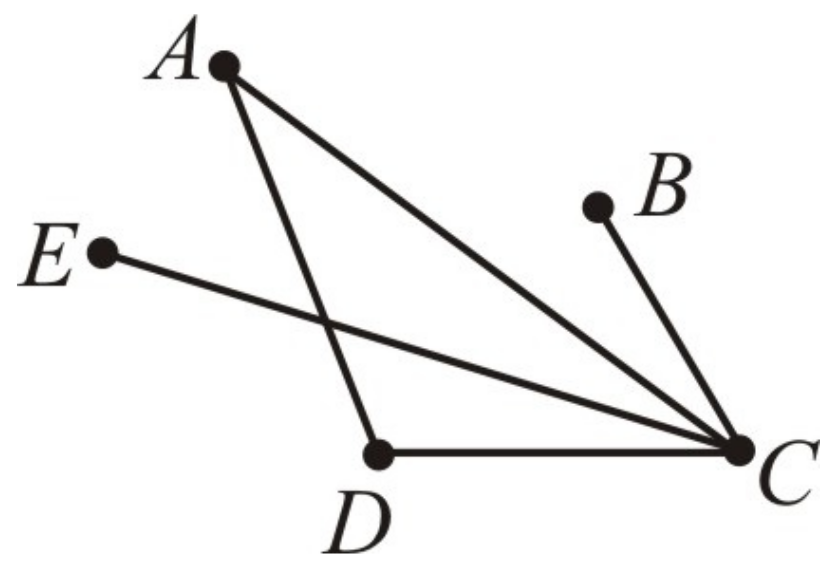
\includegraphics[scale=0.15]{../images/10.1.26.a.png}

\subsubsection{(b)}
Draw a graph that illustrates who among these five people are not acquainted. That is, draw an edge between two people if, 
and only if, they are not acquainted.

\begin{proof}
\begin{figure}[ht!]
\centering
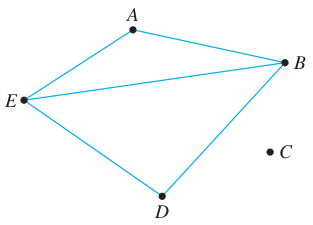
\includegraphics[scale=0.4]{../images/10.1.26.b.png}
\end{figure}
\end{proof}

\subsection{Exercise 27}
Let \(G\) be a simple graph with \(n\) vertices. What is the relation between the number of edges of \(G\) and the number 
of edges of the complement \(G'\)?

{\it Hint:} Consider the graph obtained by taking the vertices and edges of \(G\) plus all the edges of \(G'\).

\begin{proof}
\(G'\) has all the edges that \(G\) does not between any two vertices. Therefore, if we put all the edges of \(G\) and 
\(G'\) together, it should give us all possible edges between any two vertices, in other words, the complete graph \(K_n\) 
on \(n\) vertices. We know \(K_n\) has \(\frac{n(n-1)}{2}\) edges total, therefore: ``the number of edges of \(G\) plus 
the number of edges of \(G'\) equals \(\frac{n(n-1)}{2}\)''.
\end{proof}

\subsection{Exercise 28}
Show that at a party with at least two people, there are at least two mutual acquaintances or at least two mutual 
strangers.

\begin{proof}
Since there are at least 2 people at the party, consider person 1 and person 2. Either they know each other (so they 
are mutually acquainted), or they do not (so they are mutual strangers).

(This problem is stated weirdly! I have to assume that acquaintance is a symmetric relation, given Exercise 26 above: 
if person A is acquainted with person B, then person B is also acquainted with person A; in other words A cannot know B 
non-mutually without B knowing A. Otherwise, the acquaintance graph would have to be a directed graph, which has not been 
yet covered in this section.)
\end{proof}

{\bf \cy Find Hamiltonian circuits for each of the graphs in 29 and 30.}

\subsection{Exercise 29}
\begin{figure}[ht!]
\centering
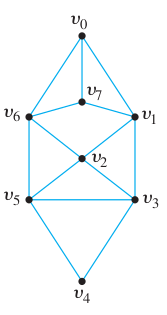
\includegraphics[scale=0.7]{../images/10.1.29.png}
\end{figure}

\begin{proof}
\(v_0 v_7 v_1 v_2 v_3 v_4 v_5 v_6 v_0\)
\end{proof}

\subsection{Exercise 30}
\begin{figure}[ht!]
\centering
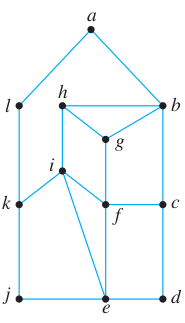
\includegraphics[scale=0.5]{../images/10.1.30.png}
\end{figure}

\begin{proof}
\(alkjedcfihgba\)
\end{proof}

{\bf \cy Show that none of the graphs in $31-33$ has a Hamiltonian circuit.}

\subsection{Exercise 31}
\begin{figure}[ht!]
\centering
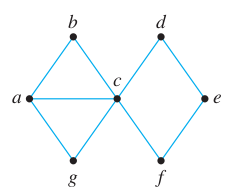
\includegraphics[scale=0.6]{../images/10.1.31.png}
\end{figure}

\begin{proof}
Argue by contradiction and assume \(G\) has a Hamiltonian circuit. By Proposition 10.1.6 \(G\) has a subgraph \(H\) that
is connected, contains every vertex of \(G\), has the same number of edges as vertices, and every vertex has degree 2.
Since vertex \(c\) has degree 5, in the subgraph \(H\) 3 of these edges must be removed. But 4 of these 5 edges cannot be
removed, otherwise \(b,d,g,f\) would have degree less than 2. This is a contradiction! So \(G\) has no Hamiltonian circuit.
\end{proof}

\subsection{Exercise 32}
\begin{figure}[ht!]
\centering
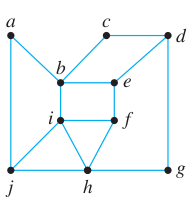
\includegraphics[scale=0.6]{../images/10.1.32.png}
\end{figure}

\begin{proof}
Call the given graph \(G\), and suppose \(G\) has a Hamiltonian circuit. Then \(G\) has a subgraph \(H\) that 
satisfies conditions (1)–(4) of Proposition 10.1.6. Since the degree of \(b\) in \(G\) is 4 and every vertex in \(H\) has 
degree 2, two edges incident on \(b\) must be removed from \(G\) to create \(H\). Edge \(\{a, b\}\) cannot be removed 
because doing so would result in vertex \(d\) having degree less than 2 in \(H\). Similar reasoning shows that edge 
\(\{b, c\}\) cannot be removed either. So edges \(\{b, i\}\) and \(\{b, e\}\) must be removed from \(G\) to create \(H\). 
Because vertex \(e\) must have degree 2 in \(H\) and because edge \(\{b, e\}\) is not in \(H\), both edges \(\{e, d\}\) and 
\(\{e, f\}\) must be in \(H\). Similarly, since both vertices \(c\) and \(g\) must have degree 2 in \(H\), edges \(\{c,d\}\) 
and \(\{g, d\}\) must also be in \(H\). But then three edges incident on \(d\), namely, \(\{e, d\}, \{c, d\}\), and 
\(\{g, d\}\), must all be in \(H\), which contradicts the fact that vertex \(d\) must have degree 2 in \(H\).
\end{proof}

\subsection{Exercise 33}
\begin{figure}[ht!]
\centering
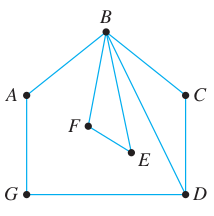
\includegraphics[scale=0.6]{../images/10.1.33.png}
\end{figure}

\begin{proof}
Similar argument to Exercises 31, 32 above. In \(H\) every vertex has degree 2. Since \(B\) has degree 5, 3 edges must be 
removed, but 4 of these 5 edges cannot be removed, otherwise \(A,F,E,C\) would have degree less than 2.
\end{proof}

{\bf \cy In $34-37$, find Hamiltonian circuits for those graphs that have them. Explain why the other graphs do not.}

\subsection{Exercise 34}
\begin{figure}[ht!]
\centering
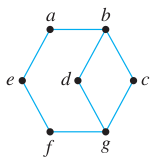
\includegraphics[scale=0.8]{../images/10.1.34.png}
\end{figure}

\begin{proof}
This graph does not have a Hamiltonian circuit. Argue like Exercises 31, 32, 33 above. In \(H\) every vertex has degree 
2. Since \(b\) has degree 3, it must have one edge removed in \(H\). But none of the 3 edges incident on \(b\) can be 
removed: otherwise one of \(a,d,c\) would have degree less than 2.
\end{proof}

\subsection{Exercise 35}
\begin{figure}[ht!]
\centering
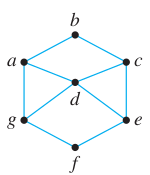
\includegraphics[scale=0.7]{../images/10.1.35.png}
\end{figure}

\begin{proof}
\(adgfecba\)
\end{proof}

\subsection{Exercise 36}
\begin{figure}[ht!]
\centering
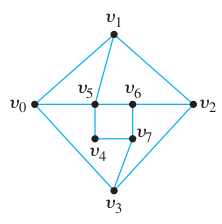
\includegraphics[scale=0.6]{../images/10.1.36.png}
\end{figure}

\begin{proof}
\(v_4v_5v_1v_0v_3v_2v_6v_7v_4\)
\end{proof}

\subsection{Exercise 37}
\begin{figure}[ht!]
\centering
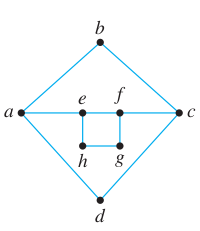
\includegraphics[scale=0.7]{../images/10.1.37.png}
\end{figure}

\begin{proof}
This graph has no Hamiltonian circuits. Similar argument as before: in \(H\) every vertex has degree 2. Since \(a\) has
degree 3, we must remove one edge. That has to be \(\{a,e\}\) otherwise \(b\) or \(d\) would have degree 1. Similarly \(c\)
has degree 3, we must remove one edge, it has to be \(\{f,c\}\) otherwise \(b\) or \(d\) would have degree 1. But after
removing those 2 edges, we are left with a disconnected graph: a ``diamond'' (\(a-b-c-d\)) with a ``square'' inside it 
(\(e-f-g-h\)), which contradicts the fact that \(H\) must be connected.
\end{proof}

\subsection{Exercise 38}
Give two examples of graphs that have Euler circuits but not Hamiltonian circuits.

\begin{proof}
One example: This graph has an Euler circuit \(v_0v_1v_2v_3v_1v_4v_0\) but no Hamiltonian circuit.

\begin{figure}[ht!]
\centering
\includegraphics[scale=0.5]{../images/10.1.38.png}
\end{figure}
\end{proof}

\subsection{Exercise 39}
Give two examples of graphs that have Hamiltonian circuits but not Euler circuits.

\begin{proof}
One example: This graph has a Hamiltonian circuit \(v_0v_1v_2v_0\) but no Euler circuit.

\begin{figure}[ht!]
\centering
\includegraphics[scale=0.5]{../images/10.1.39.png}
\end{figure}
\end{proof}

\subsection{Exercise 40}
Give two examples of graphs that have circuits that are both Euler circuits and Hamiltonian circuits.

\begin{proof}
One example: The walk \(v_0v_1v_2v_0\) is both an Euler circuit and a Hamiltonian circuit for this graph.

\begin{figure}[ht!]
\centering
\includegraphics[scale=0.5]{../images/10.1.40.png}
\end{figure}
\end{proof}

\subsection{Exercise 41}
Give two examples of graphs that have Euler circuits and Hamiltonian circuits that are not the same.

\begin{proof}
One example: This graph has the Euler circuit \(e_1e_2e_3e_4e_5e_6\) and the Hamiltonian circuit 
\(v_0v_1v_2v_3v_0\). These are not the same.

\begin{figure}[ht!]
\centering
\includegraphics[scale=0.6]{../images/10.1.41.png}
\end{figure}
\end{proof}

\subsection{Exercise 42}
\begin{figure}[ht!]
\centering
\includegraphics[scale=0.45]{../images/10.1.42.png}
\end{figure}

A traveler in Europe wants to visit each of the cities shown on the map exactly once, starting and ending in Brussels. The 
distance (in kilometers) between each pair of cities is given in the table. Find a Hamiltonian circuit that minimizes the 
total distance traveled. (Use the map to narrow the possible circuits down to just a few. Then use the table to find the 
total distance for each of those.)

\begin{proof}
Find a Hamiltonian circuit that minimizes the total distance traveled. Some possible Hamiltonian circuits are as follows:

1. Brussels-Luxembourg-Dusseldorf-Paris-Munich-Berlin-Brussels. Total distance traveled by the visitor is \(219 + 
224 + 497 + 832 + 585 + 783 = 3140\) km.

2. Brussels-Luxembourg-Paris-Munich-Berlin-Dusseldorf-Brussels. Total distance traveled by the visitor is \(219 + 
375 + 832 + 585 + 564 + 223 = 2798\) km.

3. Brussels-Paris-Luxembourg-Munich-Berlin-Dusseldorf-Brussels. Total distance traveled by the visitor is \(308 + 
375 + 517 + 585 + 564 + 223 = 2572\) km.

Therefore, the Hamiltonian circuit is Brussels-Paris-Luxembourg-Munich-Berlin- \\ Dusseldorf-Brussels in which 
total distance is minimum.
\end{proof}

\subsection{Exercise 43}
\subsubsection{(a)}
Prove that if a walk in a graph contains a repeated edge, then the walk contains a repeated vertex.

\begin{proof}
Suppose \(G\) is a graph and \(W\) is a walk in \(G\) that contains a repeated edge \(e\). Let \(v\) and \(w\) be the 
endpoints of \(e\). In case \(v = w\), then \(v\) is a repeated vertex of \(W\). In case \(v \neq w\), then one of 
the following must occur: (1) \(W\) contains two copies of \(vew\) or of \(wev\) (for instance, \(W\) might contain a 
section of the form \(vewe'vew\), as illustrated below); 

\begin{figure}[ht!]
\centering
\includegraphics[scale=0.35]{../images/10.1.43.a.png}
\end{figure}

(2) \(W\) contains separate sections of the form \(vew\) and 
\(wev\) (for instance, \(W\) might contain a section of the form \(vewe'wev\), as illustrated below); or (3) \(W\) 
contains a section of the form \(vewev\) or of the form \(wevew\) (as illustrated below). In cases (1) and (2), both 
vertices \(v\) and \(w\) are repeated, and in case (3), one of \(v\) or \(w\) is repeated. In all cases, there is at least 
one vertex in \(W\) that is repeated.
\end{proof}

\subsubsection{(b)}
Explain how it follows from part (a) that any walk with no repeated vertex has no repeated edge.

\begin{proof}
This statement is the contrapositive of part (a).
\end{proof}

\subsection{Exercise 44}
Prove Lemma 10.1.1(a): If \(G\) is a connected graph, then any two distinct vertices of \(G\) can be connected by a path. 
(You may use the result stated in exercise 43.)

\begin{proof}
Suppose \(G\) is a connected graph and \(v\) and \(w\) are any particular but arbitrarily chosen vertices of \(G\). {\it [We 
must show that \(u\) and \(v\) can be connected by a path.]} Since \(G\) is connected, there is a walk from \(v\) to \(w\). 
If the walk contains a repeated vertex, then delete the portion of the walk from the first occurrence of the vertex to 
its next occurrence. (For example, in the walk \(ve_1v_2e_5v_7e_6v_2e_3w\), the vertex \(v_2\) occurs twice. 
Deleting the portion of the walk from one occurrence to the next gives \(ve_1v_2e_3w\).) If the resulting walk still 
contains a repeated vertex, do the above deletion process another time. Then check again for a repeated vertex. Continue 
in this way until all repeated vertices have been deleted. (This must occur eventually, since the total number of 
vertices is finite.) The resulting walk connects \(v\) to \(w\) but has no repeated vertex. By exercise 43(b), it has no 
repeated edge either. Hence it is a path from \(v\) to \(w\).
\end{proof}

\subsection{Exercise 45}
Prove Lemma 10.1.1(b): If vertices \(v\) and \(w\) are part of a circuit in a graph \(G\) and one edge is removed from the 
circuit, then there still exists a trail from \(v\) to \(w\) in \(G\).

\begin{proof}
Write down the circuit as: 
\[
ve_1v_1e_2v_2 \ldots v_ne_nwf_1w_1f_2w_2 \ldots f_{m-1}w_{m-1}f_mv
\]
If one of the edges \(e_1, \ldots, e_n\) is removed then there is still a trail 
\[
wf_1w_1f_2w_2 \ldots f_{m-1}w_{m-1}f_mv
\] 
between \(w\) and \(v\), written backwards it's a trail from \(v\) to \(w\), and similarly if one of the edges \(f_1, \ldots, f_m\) is removed then there is still a trail
\[
ve_1v_1e_2v_2 \ldots v_ne_nw
\] 
from \(v\) to \(w\).
\end{proof}

\subsection{Exercise 46}
Draw a picture to illustrate Lemma 10.1.1(c): If a graph \(G\) is connected and \(G\) contains a circuit, then an edge of the 
circuit can be removed without disconnecting \(G\).

\begin{proof}
The graph below contains a circuit, any edge of which can be removed without disconnecting the graph. For instance, if edge 
\(e\) is removed, then the following walk can be used to go from \(v_1\) to \(v_2\): \(v_1v_5v_3v_2\).

\begin{figure}[ht!]
\centering
\includegraphics[scale=0.5]{../images/10.1.46.png}
\end{figure}
\end{proof}

\subsection{Exercise 47}
Prove that if there is a trail in a graph \(G\) from a vertex \(v\) to a vertex \(w\), then there is a trail from \(w\) to \(v\).

\begin{proof}
Simply traverse the trail from \(v\) to \(w\) but starting at \(w\) and going backwards. This is also a trail from 
\(w\) to \(v\) (no repeated edges).
\end{proof}

\subsection{Exercise 48}
If a graph contains a circuit that starts and ends at a vertex \(v\), does the graph contain a simple circuit that starts and 
ends at \(v\)? Why?

\begin{proof}
Yes, suppose a graph contains a circuit that starts and ends at a vertex \(v\). Successively delete sections of this 
circuit as follows. For each repeated vertex \(w\) in the circuit (excluding the first vertex if its only repetition is 
at the end of the circuit, but including the first vertex if it is repeated in the middle of the circuit), there is a 
section of the circuit of the form \(we_1v_1 \ldots e_{n-1}v_{n-1}e_n w\). Replace this section of the circuit by the 
single vertex \(w\). Because the circuit has finite length, only a finite number of such deletions can be made, after 
which a simple circuit starting and ending at will remain.
\end{proof}

\subsection{Exercise 49}
Prove that if there is a circuit in a graph that starts and ends at a vertex \(v\) and if \(w\) is another vertex in the 
circuit, then there is a circuit in the graph that starts and ends at \(w\).

\begin{proof}
If a circuit starts and ends at \(v\) and contains \(w\) then the circuit has the form
\[
ve_1v_1e_2v_2 \ldots v_ne_nwf_1w_1f_2w_2 \ldots f_{m-1}w_{m-1}f_mv.
\]
Then the following is a circuit that starts and ends at \(w\):
\[
wf_1w_1f_2w_2 \ldots f_{m-1}w_{m-1}f_mve_1v_1e_2v_2 \ldots v_ne_nw
\]
\end{proof}

\subsection{Exercise 50}
Let \(G\) be a connected graph, and let \(C\) be any circuit in \(G\) that does not contain every vertex of \(C\). Let 
\(G'\) be the subgraph obtained by removing all the edges of \(C\) from \(G\) and also any vertices that become isolated 
when the edges of \(C\) are removed. Prove that there exists a vertex \(v\) such that \(v\) is in both \(C\) and \(G'\).

\begin{proof}
Let \(G\) be a connected graph and let \(C\) be a circuit in \(G\). Let \(G'\) be the subgraph obtained by removing all the 
edges of \(C\) from \(G\) and also any vertices that become isolated when the edges of \(C\) are removed. {\it [We must 
show that there exists a vertex \(v\) such that \(v\) is in both \(C\) and \(G'\).]} Pick any vertex \(v\) of \(C\) and 
any vertex \(w\) of \(G'\). Since \(G\) is connected, there is a path from \(v\) to \(w\) (by Lemma 10.1.1(a)):
\begin{center}
\begin{tabular}{ccccccccccccccccc}
\(v\)&=&\(v_0\)&\(e_1\)&\(v_1\)&\(\cdots\)&\(e_i\)&\(v_i\)&\(e_{i+1}\)&\(v_{i+1}\)&\(\cdots\)&\(v_{n-1}\)&\(e_n\)&\(v_n\)&=&\(w\)\\
{\cy \(\uparrow\)}&&&&&&&{\cy \(\uparrow\)}&&{\cy \(\uparrow\)}&&&&&&{\cy \(\uparrow\)}\\
{\cy in \(C\)}&&&&&&&{\cy in \(C\)}&&{\cy not in \(C\)}&&&&&&{\cy in \(G'\)}
\end{tabular}
\end{center}
Let \(i\) be the largest subscript such that \(v_i\) is in \(C\). If \(i = n\), then \(v_n = w\) is in \(C\) and also in 
\(G'\), and we are done. If \(i < n\), then \(v_i\) is in \(C\) and \(v_i + 1\) is not in \(C\). This implies that \(e_i 
+ 1\) is not in \(C\) (for if it were, both endpoints would be in \(C\) by definition of circuit). Hence when \(G'\) is 
formed by removing the edges and resulting isolated vertices from \(G\), then \(e_i + 1\) is not removed. That means that 
\(v_i\) does not become an isolated vertex, so \(v_i\) is not removed either. Hence \(v_i\) is in \(G'\). Consequently, 
\(v_i\) is in both \(C\) and \(G'\) {\it [as was to be shown].}
\end{proof}

\subsection{Exercise 51}
Prove that any graph with an Euler circuit is connected.

\begin{proof}
Suppose \(G\) is a graph with an Euler circuit. If \(G\) has only one vertex, then \(G\) is automatically connected. If 
\(v\) and \(w\) are any two vertices of \(G\), then \(v\) and \(w\) each appear at least once in the Euler circuit (since an 
Euler circuit contains every vertex of the graph). The section of the circuit between the first occurrence of one of \(v\) or 
\(w\) and the first occurrence of the other is a walk from one of the two vertices to the other. Since the choice of \(v\) 
and \(w\) was arbitrary, given any two vertices in \(G\) there is a walk from one to the other. So, by definition, 
\(G\) is connected.
\end{proof}

\subsection{Exercise 52}
Prove Corollary 10.1.5.

{\it Corollary:} Let \(G\) be a graph, and let \(v\) and \(w\) be two distinct vertices of \(G\). There is an Euler trail 
from \(v\) to \(w\) if, and only if, \(G\) is connected, \(v\) and \(w\) have odd degree, and all other vertices of \(G\) 
have positive even degree.

\begin{proof}
\(\bm{(\implies)}\) Assume there is an Euler trail from \(v\) to \(w\). 

Then this trail passes through every vertex of \(G\) at least once and traverses every edge of \(G\) exactly once, therefore 
\(G\) is connected. Adding an extra edge \(e\) between \(v\) and \(w\) to this trail gives us an Euler circuit. Then every 
vertex in this new graph has even degree. Removing \(e\) shows that \(v\) and \(w\) have odd degree and all other vertices 
have even degree in the original graph \(G\).

\(\bm{(\impliedby)}\) Assume \(G\) is connected, \(v\) and \(w\) have odd degree, and all other vertices of \(G\) have 
positive even degree.

Add an extra edge \(e\) between \(v\) and \(w\). Now every vertex in this new graph has even degree, and it is connected.
So it has an Euler circuit by Theorem 10.1.4. This Euler circuit contains \(e\). Removing \(e\) from the circuit gives
us an Euler trail from \(v\) to \(w\) in the original graph \(G\).
\end{proof}

\subsection{Exercise 53}
For what values of \(n\) does the complete graph \(K_n\) with \(n\) vertices have (a) an Euler circuit? (b) a Hamiltonian 
circuit? Justify your answers.

\begin{proof}
\(K_n\) has a circuit if and only if \(n \geq 3\).

(a) Euler circuits require a connected graph where every vertex has even degree. Every vertex in \(K_n\) has degree 
\(n-1\). So this means that for all \(n\), \(K_n\) has an Euler circuit if and only if \(n \geq 3\) and \(n\) is odd.

(b) Hamiltonian circuits require a connected subgraph \(H\) with the same number of edges and vertices, which contains 
every vertex of \(G\), such that every vertex has degree 2 in \(H\). This is possible in every \(K_n\) with \(n \geq 3\). If
the vertices are \(v_1, \ldots, v_n\) then let \(H\) be \(v_1v_2\cdots v_{n-1}v_nv_1\). This is a connected circuit 
with \(n\) vertices and \(n\) edges, where every vertex has degree 2.
\end{proof}

\subsection{Exercise 54}
For what values of \(m\) and \(n\) does the complete bipartite graph on \((m, n)\) vertices have (a) an Euler circuit? (b) a 
Hamiltonian circuit? Justify your answers.

\begin{proof}
(a) Euler circuit requires every vertex to have even degree, and in \(K_{m,n}\) the left \(m\) vertices all have degree 
\(n\) and the right \(n\) vertices all have degree \(m\). So \(K_{m,n}\) has an Euler circuit if and only if both \(m\) and
\(n\) are even (and \(\geq 2\)).

(b) Hamiltonian circuit requires every vertex to have degree 2. The total degree of the left \(m\) vertices is \(2m\), so
there are \(2m\) edges going from the left \(m\) vertices to the right \(n\) vertices, covering a total degree of \(2n\) on
the right. This forces \(2m = 2n\) so \(m=n\). So \(K_{m,n}\) has a Hamiltonian circuit if and only if \(m=n\) (and \(\geq 2\)).
\end{proof}

\subsection{Exercise 55}
What is the maximum number of edges a simple disconnected graph with \(n\) vertices can have? Prove your answer.

\begin{proof}
Simple means no loops or parallel edges. Leave out 1 vertex by itself so it's not connected to any of the other \(n-1\). Now
we try to find the maximum number of edges we can have among the \(n-1\) vertices without introducing any loops. We can add
\(n-2\) edges between them in a chain. Adding 1 more edge to this would create a loop. So the maximum is \(n-2\).
\end{proof}

\subsection{Exercise 56}
\subsubsection{(a)}
Prove that if \(G\) is any bipartite graph, then every circuit in \(G\) has an even number of edges.

\begin{proof}
Let \(G = (V_1, V_2)\) be a bipartite graph where \(V_1\) is the set of vertices on the left and \(V_2\) is the set of 
vertices on the right. Consider any circuit. Say, it starts and ends at a vertex \(v \in V_1\). Since \(v\) can only be 
connected to vertices in \(V_2\), one edge brings us to \(V_2\). Similarly, since vertices in \(V_2\) can only be 
connected to vertices in \(V_1\), the second edge of the circuit brings us back to \(V_1\). And so on. Any odd number 
of edges starting from \(v\) will end in \(V_2\), unable to complete the circuit back at \(v\). Hence, no circuit can have
an odd number of edges, but must have an even number of edges.
\end{proof}

\subsubsection{(b)}
Prove that if \(G\) is any graph with at least two vertices and if \(G\) does not have a circuit with an odd number of 
edges, then \(G\) is bipartite.

{\it Hint:} Divide the proof into three parts. (1) Show that if \(G\) is any graph containing a closed walk with an odd 
number of edges, then \(G\) contains a circuit with an odd number of edges. (2) Show that if \(G\) is any connected graph 
that does not have a circuit with an odd number of edges, then \(G\) is bipartite. (3) Show that if \(G\) is any graph with 
at least two vertices and is such that \(G\) does not have a circuit with an odd number of edges, then \(G\) is bipartite.

\begin{proof}
(1) Let \(W\) be a closed walk with an odd number of edges. If no vertices are repeated in \(W\) then \(W\) is already a 
circuit with an odd number of edges. So suppose \(W\) has a repeated vertex. Write \(W = v_1v_2 \cdots v_jv_{j+1} \cdots 
v_kv_{k+1} \cdots v_nv_1\) where \(v_j = v_k\) is the repeated vertex. Now \(W\) is the union of two closed walks: \(v_1v_2 
\cdots v_jv_{k+1} \cdots v_n\) and \(v_jv_{j+1} \cdots v_k\). Since the number of edges of \(W\) is odd, and the sum of the 
numbers of edges of these two walks equals the number of edges of \(W\), one of these two walks must have an odd number of 
edges and the other must have an even number of edges (because odd + odd = even, even + even = even, and only odd + even = 
odd). Take the walk among the two walks that has the odd number of edges. Either this smaller walk is a circuit, or it 
also has a repeated vertex. Then repeat the procedure to obtain an even smaller closed walk with an odd number of 
edges. The process eventually terminates since \(W\) is finite. So there is a circuit with an odd number of edges.

(2) Assume \(G\) is connected and has no circuit with an odd number of edges. Let \(v\) be a vertex in \(G\). Since \(G\)
is connected, there is a walk between \(v\) and any other vertex. For any vertex \(w\) let \(d(w, v)\) denote the length 
of the shortest walk between \(v\) and \(w\). Let's define a bipartition of \(G\) as follows: 
\[
V_1 = \{w \in V(G) \, | \, d(w, v) \text{ is odd}\}, \,\,\, V_2 = \{w \in V(G) \, | \, d(w, v) \text{ is even}\}
\]
We need to prove \((V_1, V_2)\) is a bipartition of \(G\). Argue by contradiction and assume \(x,y \in V_1\) and assume
there is an edge \(e\) between \(x\) and \(y\). Now there is a closed walk with an odd number of edges from \(v\) to \(v\) as 
follows: start with a walk from \(v\) to \(x\) which has odd length (since \(x \in V_1\)), followed by \(e\) (add 1), 
followed by the walk from \(y\) to \(v\) which has odd length. This is a closed walk of odd length, which, by (1), implies
there is a circuit of odd length from \(v\) to \(v\), which is a contradiction to the assumption that \(G\) has no circuits
of odd length. Similar argument for \(V_2\).

(3) Assume \(G\) is any graph with at least two vertices and has no circuit with an odd number of edges. Consider all the
connected components \(G_1, \ldots, G_n\) of \(G\). By (2) each \(G_i\) is bipartite: \(G_i = (V_{1,i}, V_{2,i})\). Then 
we can create a bipartition of \(G\): \((\bigcup_{i=1}^n V_{1,i}, \bigcup_{i=1}^n V_{2,i})\). So \(G\) is bipartite.
\end{proof}

\subsection{Exercise 57}
An alternative proof for Theorem 10.1.3 has the following outline. Suppose \(G\) is a connected graph in which every 
vertex has even degree. Suppose the trail \\ \(C: v_1e_1v_2e_2v_3 \ldots e_nv_{n+1}\) has maximum length in 
\(G\). That is, \(C\) has at least as many vertices and edges as any other trail in \(G\). First derive a contradiction from 
the assumption that \(v_1 \neq v_{n+1}\). Next let \(H\) be the subgraph of \(G\) that contains all the vertices and edges 
in \(C\). Then derive a contradiction from the assumption that \(H \neq G\). Show that \(H\) contains every vertex of \(G\), 
and show that \(H\) contains every edge of \(G\).

\begin{proof}
Argue by contradiction and assume \(v_1 \neq v_{n+1}\). Note that \(v_1\) is connected to only one other vertex, \(v_2\), 
on \(C\), and \(v_{n+1}\) is connected to only one other vertex, \(v_n\), in \(C\). Since both \(v_1\) and \(v_{n+1}\)
have even degree, they have degree at least 2. So they are connected to at least one more vertex. Then there is a trail 
in \(G\) longer than \(C\), contradiction. So \(v_1 = v_{n+1}\).

Let \(H\) be the subgraph of \(G\) that contains all the vertices and edges in \(C\). Argue by contradiction and assume
\(H \neq G\). First assume \(G\) has a vertex \(w\) that \(H\) does not. Since \(w\) is different than all \(v_1, \ldots, 
v_n\), \(w\) is not on \(C\). Since \(G\) is connected there is a trail from \(v_1\) to \(w\). Since \(w\) is not on \(C\), 
this trail is not part of \(C\). Adding this trail to \(C\) gives us a longer trail, contradiction. So \(H\) contains 
every vertex of \(G\). 

Now assume \(G\) has an edge \(e\) that \(H\) does not. This edge must be connecting two of the vertices \(v_1, \ldots, 
v_n\). Say \(v_i\) and \(v_j\). But then \(v_i\) and \(v_j\) have degree 3, contradiction. So \(H\) contains every edge 
of \(G\).
\end{proof}

\section{Exercise Set 10.2}
\subsection{Exercise 1}
Find real numbers a, b, and c such that the following are true.

\subsubsection{(a)}
\(
\left[ 
\begin{array}{cc}
a + b & a - c \\
c & b - a \\
\end{array}
\right] = 
\left[ 
\begin{array}{rr}
1 & 0 \\
-1 & 3 \\
\end{array}
\right]
\)
{\it Proof.} \(c=-1, a=-1, b=2\)

\subsubsection{(b)}
\[
\left[ 
\begin{array}{cc}
2a & b + c \\
c - a & 2b - a \\
\end{array}
\right] = 
\left[ 
\begin{array}{rr}
4 & 3 \\
1 & -2 \\
\end{array}
\right]
\]
\begin{proof}
\(a=2, c=3, b=0\)
\end{proof}

\subsection{Exercise 2}
Find the adjacency matrices for the following directed graphs.

\subsubsection{(a)}
\includegraphics[scale=0.6]{../images/10.2.2.a.1.png}
{\it Proof.}
\includegraphics[scale=0.6]{../images/10.2.2.a.png}

\subsubsection{(b)}
\includegraphics[scale=0.6]{../images/10.2.2.b.1.png}
{\it Proof.}
\begin{tabular}{ccccc}
 & {\cy \(v_1\)} & {\cy \(v_2\)} & {\cy \(v_3\)} & {\cy \(v_4\)} \\
{\cy \(v_1\)} & 1 & 0 & 1 & 0 \\
{\cy \(v_2\)} & 0 & 0 & 1 & 0 \\
{\cy \(v_3\)} & 1 & 0 & 0 & 1 \\
{\cy \(v_4\)} & 0 & 0 & 1 & 0 \\
\end{tabular}

\subsection{Exercise 3}
Find directed graphs that have the following adjacency matrices:

\subsubsection{(a)}
\(
\left[ 
\begin{array}{cccc}
1 & 0 & 1 & 2 \\
0 & 0 & 1 & 0 \\
0 & 2 & 1 & 1 \\
0 & 1 & 1 & 0 \\
\end{array}
\right]
\)
{\it Proof.} \includegraphics[scale=0.5]{../images/10.2.3.a.png}

\subsubsection{(b)}
\(
\left[ 
\begin{array}{cccc}
0 & 1 & 0 & 0 \\
2 & 0 & 1 & 0 \\
1 & 2 & 1 & 0 \\
0 & 0 & 1 & 0 \\
\end{array}
\right]
\)
{\it Proof.} \includegraphics[scale=0.4]{../images/10.2.3.b.png}

\subsection{Exercise 4}
Find adjacency matrices for the following (undirected) graphs.

\subsubsection{(a)}
\includegraphics[scale=0.6]{../images/10.2.4.a.1.png}
{\it Proof.}
\includegraphics[scale=0.6]{../images/10.2.4.a.png}

\subsubsection{(b)}
\includegraphics[scale=0.6]{../images/10.2.4.b.1.png}
{\it Proof.}
\begin{tabular}{ccccc}
 & {\cy \(v_1\)} & {\cy \(v_2\)} & {\cy \(v_3\)} & {\cy \(v_4\)} \\
{\cy \(v_1\)} & 1 & 0 & 0 & 0 \\
{\cy \(v_2\)} & 0 & 1 & 1 & 2 \\
{\cy \(v_3\)} & 0 & 1 & 1 & 0 \\
{\cy \(v_4\)} & 0 & 2 & 0 & 0 \\
\end{tabular}

\subsubsection{(c)}
\(K_4\), the complete graph on four vertices
{\it Proof.} \includegraphics[scale=0.6]{../images/10.2.4.c.png}

\subsubsection{(d)}
\(K_{2,3}\), the complete bipartite graph on (2, 3) vertices
{\it Proof.}
\begin{tabular}{cccccc}
 & {\cy \(v_1\)} & {\cy \(v_2\)} & {\cy \(v_3\)} & {\cy \(w_1\)} & {\cy \(w_2\)} \\
{\cy \(v_1\)} & 0 & 0 & 0 & 1 & 1 \\
{\cy \(v_2\)} & 0 & 0 & 0 & 1 & 1 \\
{\cy \(v_3\)} & 0 & 0 & 0 & 1 & 1 \\
{\cy \(w_1\)} & 1 & 1 & 1 & 0 & 0 \\
{\cy \(w_2\)} & 1 & 1 & 1 & 0 & 0 \\
\end{tabular}

\subsection{Exercise 5}
Find graphs that have the following adjacency matrices.

\subsubsection{(a)}
\(
\left[ 
\begin{array}{ccc}
1 & 0 & 1 \\
0 & 1 & 2 \\
1 & 2 & 0 \\
\end{array}
\right]
\)
{\it Proof.} \includegraphics[scale=0.6]{../images/10.2.5.a.png}

\subsubsection{(b)}
\(
\left[ 
\begin{array}{ccc}
0 & 2 & 0 \\
2 & 1 & 0 \\
0 & 0 & 1 \\
\end{array}
\right]
\)
{\it Proof.} \includegraphics[scale=0.6]{../images/10.2.5.b.png}

\subsection{Exercise 6}
The following are adjacency matrices for graphs. In each case determine whether the graph is connected by analyzing the 
matrix without drawing the graph.

\subsubsection{(a)}
\[
\left[ 
\begin{array}{ccc}
0 & 1 & 1 \\
1 & 1 & 0 \\
1 & 0 & 0 \\
\end{array}
\right]
\]
\begin{proof}
From the first row, we see that \(v_1\) is adjacent to \(v_2\) and \(v_3\). Therefore the graph is connected.
\end{proof}

\subsubsection{(b)}
\[
\left[ 
\begin{array}{cccc}
0 & 2 & 0 & 0 \\
2 & 0 & 0 & 0 \\
0 & 0 & 1 & 1 \\
0 & 0 & 1 & 1 \\
\end{array}
\right]
\]
\begin{proof}
From the first two rows, we can see there are 2 edges between \(v_1\) and \(v_2\). From the last two rows, we can see that
\(v_3\) and \(v_4\) are adjacent. However, there are no edges between the \(v_1+v_2\) connected component and the 
\(v_3+v_4\) connected component. Thus the graph is disconnected.
\end{proof}

\subsection{Exercise 7}
Suppose that for every positive integer \(i\), all the entries in the \(i\)th row and \(i\)th column of the adjacency matrix 
of a graph are 0. What can you conclude about the graph?

\begin{proof}
The \(i\)th row and column defines the edges between \(v_i\) and the other vertices. If the entries are all 0, that means
there are no edges between \(v_i\) and the other vertices. So the graph is not connected; \(v_i\) is disconnected from the
rest of the graph.
\end{proof}

\subsection{Exercise 8}
Find each of the following products.

\subsubsection{(a)}
\[
\left[ 
\begin{array}{rr}
2 & -1 \\
\end{array}
\right]
\left[ 
\begin{array}{c}
1 \\
3
\end{array}
\right]
\]
\begin{proof}
\(2 \cdot 1 + (-1) \cdot 3 = -1\)
\end{proof}

\subsubsection{(b)}
\[
\left[ 
\begin{array}{rrr}
4 & -1 & 7 \\
\end{array}
\right]
\left[ 
\begin{array}{c}
1 \\
2 \\
0
\end{array}
\right]
\]
\begin{proof}
\(4 \cdot 1 + (-1) \cdot 2 + 7 \cdot 0 = 2\)
\end{proof}

\subsection{Exercise 9}
Find each of the following products.

\subsubsection{(a)}
\[
\left[ 
\begin{array}{rr}
3 & 0 \\
1 & -2 \\
\end{array}
\right]
\left[ 
\begin{array}{rrr}
1 & -1 & 4 \\
0 & 2 & 1 \\
\end{array}
\right]
\]
\begin{proof}
\(\left[ 
\begin{array}{rrr}
3 & -3 & 12 \\
1 & -5 & 2 \\
\end{array}
\right]\)
\end{proof}

\subsubsection{(b)}
\[
\left[ 
\begin{array}{rrr}
2 & 0 & 1 \\
0 & -1 & 0 \\
\end{array}
\right]
\left[ 
\begin{array}{rr}
1 & 3 \\
5 & -4 \\
-2 & 2 \\
\end{array}
\right]
\]
\begin{proof}
\(\left[ 
\begin{array}{rr}
0 & 8 \\
-5 & 4 \\
\end{array}
\right]\)
\end{proof}

\subsubsection{(c)}
\[
\left[ 
\begin{array}{r}
-1 \\
2 \\
\end{array}
\right]
\left[ 
\begin{array}{rr}
2 & 3 \\
\end{array}
\right]
\]
\begin{proof}
\(\left[ 
\begin{array}{rr}
-2 & -3 \\
4 & 6 \\
\end{array}
\right]\)
\end{proof}

\subsubsection{(d)}
\[
\left[ 
\begin{array}{rr}
1 & 2 \\
3 & -1 \\
\end{array}
\right]^2
\]
\begin{proof}
\(\left[ 
\begin{array}{rr}
7 & 0 \\
0 & 7 \\
\end{array}
\right]\)
\end{proof}

\subsection{Exercise 10}
Let \({\bf A} = 
\left[ 
\begin{array}{rrr}
1 & 1 & -1 \\
0 & -2 & 1 \\
\end{array}
\right]
\), \({\bf B} = 
\left[ 
\begin{array}{rr}
-2 & 0 \\
1 & 3 \\
\end{array}
\right]
\), and \({\bf C} = 
\left[ 
\begin{array}{rr}
0 & -2 \\
3 & 1 \\
1 & 0 \\
\end{array}
\right]
\). For each of the following, determine whether the indicated product exists, and compute it if it does.

\subsubsection{(a)}
{\bf AB}\hspace{3cm}
{\it Proof.}
No product. ({\bf A} has three columns, and {\bf B} has two rows.)

\subsubsection{(b)}
{\bf BA}\hspace{3cm}
{\it Proof.}
\({\bf BA} = 
\left[ 
\begin{array}{rrr}
-2 & -2 & 2 \\
1 & -5 & 2 \\
\end{array}
\right]
\)

\subsubsection{(c)}
\({\bf A^2}\)
\begin{proof}
No product. ({\bf A} has different numbers of rows and columns.)
\end{proof}

\subsubsection{(d)}
{\bf BC}
\begin{proof}
No product. ({\bf B} has 2 columns, {\bf C} has 3 rows.)
\end{proof}

\subsubsection{(e)}
{\bf CB}\hspace{3cm}
{\it Proof.}
\({\bf CB} = 
\left[ 
\begin{array}{rr}
-2 & -6 \\
-5 & 3 \\
-2 & 0 \\
\end{array}
\right]
\)

\subsubsection{(f)}
\({\bf B^2}\)\hspace{3cm}
{\it Proof.}
\({\bf B^2} = 
\left[ 
\begin{array}{rr}
4 & 0 \\
1 & 9 \\
\end{array}
\right]
\)

\subsubsection{(g)}
\({\bf B^3}\)\hspace{3cm}
{\it Proof.}
\({\bf B^3} = 
\left[ 
\begin{array}{rr}
-8 & 0 \\
7 & 27 \\
\end{array}
\right]
\)

\subsubsection{(h)}
\({\bf C^2}\)\hspace{3cm}
{\it Proof.} No product. ({\bf C} has different numbers of rows and columns.)

\subsubsection{(i)}
{\bf AC}\hspace{3cm}
{\it Proof.}
\({\bf AC} = 
\left[ 
\begin{array}{rr}
2 & -1 \\
-5 & -2 \\
\end{array}
\right]
\)

\subsubsection{(j)}
{\bf CA}\hspace{3cm}
{\it Proof.}
\({\bf CA} = 
\left[ 
\begin{array}{rrr}
0 & 4 & -2 \\
3 & 1 & -2\\
1 & 1 & -1 \\
\end{array}
\right]
\)

\subsection{Exercise 11}
Give an example different from that in the text to show that matrix multiplication is not commutative. That is, find 
\(2 \times 2\) matrices {\bf A}\, and {\bf B}\, such that {\bf AB} and {\bf BA} both exist but \({\bf AB} \neq {\bf BA}\).

\begin{proof}
\({\bf A} = 
\left[ 
\begin{array}{rr}
1 & 2 \\
3 & 4 \\
\end{array}
\right], {\bf B} = 
\left[ 
\begin{array}{rr}
2 & 4 \\
3 & 6 \\
\end{array}
\right], {\bf AB} = 
\left[ 
\begin{array}{rr}
8 & 16 \\
18 & 36 \\
\end{array}
\right], {\bf BA} = 
\left[ 
\begin{array}{rr}
14 & 20 \\
21 & 30 \\
\end{array}
\right], {\bf AB} \neq {\bf BA}.
\)
\end{proof}

\subsection{Exercise 12}
Let O denote the matrix 
\(\left[ 
\begin{array}{rr}
0 & 0 \\
0 & 0 \\
\end{array}
\right]
\). Find \(2 \times 2\) matrices {\bf A} and {\bf B} such that {\bf A} \(\neq\) O and {\bf B} \(\neq\) O but {\bf AB} = O.

\begin{proof}
One among many possible examples is 
\({\bf A} = {\bf B} =
\left[ 
\begin{array}{rr}
0 & 1 \\
0 & 0 \\
\end{array}
\right]
\).
\end{proof}

\subsection{Exercise 13}
Let O denote the matrix 
\(\left[ 
\begin{array}{rr}
0 & 0 \\
0 & 0 \\
\end{array}
\right]
\). Find \(2 \times 2\) matrices {\bf A} and {\bf B} such that {\bf A} \(\neq\) {\bf B}, {\bf B} \(\neq\) O and {\bf AB} \(\neq\) O but 
{\bf BA} = O.

\begin{proof}
\({\bf A} = 
\left[ 
\begin{array}{rr}
1 & 0 \\
0 & 0 \\
\end{array}
\right],
{\bf B} =
\left[ 
\begin{array}{rr}
0 & 1 \\
0 & 0 \\
\end{array}
\right]
\). Then {\bf A} \(\neq\) {\bf B} \(\neq\) O, {\bf AB} = {\bf B} \(\neq\) O, but {\bf BA} = O.
\end{proof}

{\bf \cy In \(14-18\), assume the entries of all matrices are real numbers.}

\subsection{Exercise 14}
Prove that if {\bf I} is the \(m \times m\) identity matrix and {\bf A} is any \(m \times n\) matrix, then \({\bf IA = A}\).

\begin{proof}
We need to show that for all \(1 \leq i \leq m\) and all \(1 \leq j \leq m\), \({\bf (IA)}_{ij} = {\bf A}_{ij}\). In other 
words, we need to show that {\bf IA} and {\bf A} have the same  entries.

Denote the entries of {\bf I} by \(\delta_{ik}\). The identity matrix has 1's only on the diagonal and 0's elsewhere. Thus
\(
\delta_{ik} =
\left\{
\begin{tabular}{ll}
1 & if \(i = k\) \\
0 & if \(i \neq k\)
\end{tabular}
\right.
\). Now by the multiplication formula, \({\bf(IA)}_{ij} = \sum_{k=1}^m {\bf I}_{ik} {\bf A}_{kj} = \sum_{k=1}^m \delta_{ik} 
{\bf A}_{kj} = {\bf A}_{ij}\) because all the terms in the sum are 0 except when \(k=i\), {\it [as was to be shown]}.
\end{proof}

\subsection{Exercise 15}
Prove that if {\bf A} is an \(m \times m\) symmetric matrix, then \({\bf A^2}\) is symmetric.

\begin{proof}
Suppose {\bf A} is an \(m \times m\) symmetric matrix. Then for all integers \(i\) and \(j\) with \(1 \leq i, j \leq m\),
\[
{\bf A}^2_{ij} = \sum_{k=1}^{m} {\bf A}_{ik} {\bf A}_{kj} \text{ and } {\bf A}^2_{ji} = \sum_{k=1}^{m} {\bf A}_{jk} {\bf A}_{ki}
\]
But since {\bf A} is symmetric, \({\bf A}_{ik} = {\bf A}_{ki}\) and \({\bf A}_{kj} = {\bf A}_{jk}\) for all \(i, j\), and \(k\), and thus \({\bf A}_{ik}
{\bf A}_{kj} = {\bf A}_{jk} {\bf A}_{ki}\) {\it [by the commutative law for multiplication of real numbers]}. Hence \(({\bf A}^2)_{ij} = 
({\bf A}^2)_{ji}\) for all integers \(i\) and \(j\) with \(1 \leq i, j \leq m\).
\end{proof}

\subsection{Exercise 16}
Prove that matrix multiplication is associative: If {\bf A}, {\bf B}, and {\bf C} are any \(m \times k, k \times r\), and 
\(r \times n\) matrices, respectively, then ({\bf A}{\bf B}){\bf C} = {\bf A}({\bf B}{\bf C}). 
({\it Hint:} Summation notation is helpful.)

\begin{proof}
{\bf A}{\bf B} is an \(m \times r\) matrix, where the \(ij^{th}\) entry is \({\bf A}{\bf B}_{ij} = \sum_{x=1}^{k}{\bf A}_{ix}{\bf B}_{xj}\).

{\bf B}{\bf C} is an \(k \times n\) matrix, where the \(ij^{th}\) entry is \({\bf B}{\bf C}_{ij} = \sum_{y=1}^{r}{\bf B}_{iy}{\bf C}_{yj}\).

({\bf A}{\bf B}){\bf C} is an \(m \times n\) matrix, where the \(ij^{th}\) entry is \([({\bf A}{\bf B}){\bf C}]_{ij} = 
\sum_{y=1}^{r} ({\bf A}{\bf B})_{iy}{\bf C}_{yj} = \)
\[
\sum_{y=1}^{r} \left(\sum_{x=1}^{k}{\bf A}_{ix}{\bf B}_{xy}\right) {\bf C}_{yj} 
= \sum_{y=1}^{r}\left(\sum_{x=1}^{k}{\bf A}_{ix}{\bf B}_{xy} {\bf C}_{yj}\right)
= \sum_{x=1}^{k}{\bf A}_{ix}\left(\sum_{y=1}^{r}{\bf B}_{xy} {\bf C}_{yj}\right)
\]
(notice we are allowed to switch the order of the summation since this is a finite sum).

{{\bf A}({\bf B}{\bf C})} is an \(m \times n\) matrix, where the \(ij^{th}\) entry is \([{\bf A}({\bf B}{\bf C})]_{ij} = 
\sum_{x=1}^{k} {\bf A}_{ix}({\bf B}{\bf C})_{xj}= \)
\[
\sum_{x=1}^{k}{\bf A}_{ix}\left(\sum_{y=1}^{r}{\bf B}_{xy}{\bf C}_{yj}\right)
\]
{\it [as was to be shown.]}
\end{proof}

\subsection{Exercise 17}
Use mathematical induction and the result of exercise 16 to prove that if {\bf A} is any \(m \times m\) matrix, then \({\bf A^n A = AA^n}\) for each integer \(n \geq 1\).

\begin{proof}
Let the property \(P(n)\) be the equation \({\bf A}^n {\bf A} = {\bf A}{\bf A}^n\).

{\bf Show that \(P(1)\) is true:} We must show that \({\bf A}^1{\bf A} = {\bf A}{\bf A}^1\). But this is true because 
\({\bf A}^1 = {\bf A}\) and \({\bf A}{\bf A} = {\bf A}{\bf A}\).

{\bf Show that for every integer \(k \geq 1\), if \(P(k)\) is true, then \(P(k + 1)\) is true:} Let \(k\) be any integer 
such that \(k \geq 1\), and suppose that \({\bf A}^k{\bf A} = {\bf A}{\bf A}^k\). {\it [This is the inductive hypothesis.]} 
We must show that \({\bf A}^{k+1}{\bf A} = {\bf A}{\bf A}^{k+1}\). But
\begin{center}
\begin{tabular}{rcll}
\({\bf A}^{k+1}{\bf A}\) & = & \(({\bf A}{\bf A}^k){\bf A}\) & {\cy by definition of matrix power} \\
& = & \({\bf A}({\bf A^k}{\bf A})\) & {\cy by exercise 16} \\
& = & \({\bf A}({\bf A}{\bf A}^k)\) & {\cy by inductive hypothesis} \\
& = & \({\bf A}{\bf A}^{k+1}\) & {\cy by definition of matrix power} \\
\end{tabular}
\end{center}
\end{proof}

\subsection{Exercise 18}
Use mathematical induction to prove that if {\bf A} is an \(m \times m\) symmetric matrix, then for any integer 
\(n \geq 1\), \({\bf A}^n\) is also symmetric.

\begin{proof}
Let the property \(P(n)\) be the statement ``\({\bf A}^n\) is symmetric''.

{\bf Show that \(P(1)\) is true:} We must show that \({\bf A}^1\) is symmetric. But this is true because 
\({\bf A}^1 = {\bf A}\) and {\bf A} is symmetric by assumption.

{\bf Show that for every integer \(k \geq 1\), if \(P(k)\) is true, then \(P(k + 1)\) is true:} Let \(k\) be any integer 
such that \(k \geq 1\), and suppose that \({\bf A}^k\) is symmetric. {\it [This is the inductive hypothesis.]} 
We must show that \({\bf A}^{k+1}\) is symmetric. 

Since \({\bf A}^{k+1} = {\bf A}{\bf A}^k\), the \(ij^{th}\) entry in \({\bf A}^{k+1}\) is, by definition of matrix 
multiplication \(\sum_{l=1}^m {\bf A}_{il} ({\bf A}^k)_{lj}\). Similarly the \(ji^{th}\) entry in \({\bf A}^{k+1}\) is
\(\sum_{l=1}^m {\bf A}_{jl} ({\bf A}^k)_{li}\). We need to show these two are equal.

By exercise 17, \({\bf A}{\bf A}^k = {\bf A}^k{\bf A}\). This means that the \(ij^{th}\) entries in both of these products 
are the same. So \(\sum_{l=1}^m{\bf A}_{il} ({\bf A}^k)_{lj}\) is the same as \(\sum_{l=1}^m ({\bf A}^k)_{il}{\bf A}_{lj}\).
By the inductive hypothesis \(({\bf A}^k)_{il} = ({\bf A}^k)_{li}\), and since {\bf A} is symmetric, \({\bf A}_{lj} = 
{\bf A}_{jl}\). Putting all these facts together, we see that \(\sum_{l=1}^m {\bf A}_{il} ({\bf A}^k)_{lj}\) is the same as
\(\sum_{l=1}^m {\bf A}_{jl} ({\bf A}^k)_{li}\), {\it [as was to be shown.]}
\end{proof}

\subsection{Exercise 19}
\subsubsection{(a)}
Let \({\bf A} = 
\left[ 
\begin{array}{rrr}
1 & 1 & 2 \\
1 & 0 & 1\\
2 & 1 & 0 \\
\end{array}
\right]
\). Find \({\bf A}^2\) and \({\bf A}^3\).

\begin{proof}
\({\bf A}^2 = 
\left[ 
\begin{array}{rrr}
6 & 3 & 3 \\
3 & 2 & 2 \\
3 & 2 & 5 \\
\end{array}
\right]
\), 
\({\bf A}^3 = 
\left[ 
\begin{array}{rrr}
15 & 9 & 15 \\
9 & 5 & 8 \\
15 & 8 & 8 \\
\end{array}
\right]
\)
\end{proof}

\subsubsection{(b)}
Let \(G\) be the graph with vertices \(v_1, v_2\), and \(v_3\) and with \(A\) as its adjacency matrix. Use the answers to 
part (a) to find the number of walks of length 2 from \(v_1\) to \(v_3\) and the number of walks of length 3 from \(v_1\) to 
\(v_3\). Do not draw \(G\) to solve this problem.

\begin{proof}
By Theorem 10.2.2, there are 3 walks of length 2 and 15 walks of length 3. (top-right or bottom-left entry)
\end{proof}

\subsubsection{(c)}
Examine the calculations you performed in answering part (a) to find five walks of length 2 from \(v_3\) to \(v_3\). Then 
draw \(G\) and find the walks by visual inspection.

\begin{proof}
In {\bf A} looking at the third row we see there are 2 edges between \(v_1\) and \(v_3\), call them \(e_3, e_4\), and 1 
edge between \(v_2\) and \(v_3\), call it \(e_2\). We can use these to form length 2 walks from \(v_3\) to \(v_3\): 
\(v_3e_3v_1e_3v_3\), \(v_3e_3v_1e_4v_3\), \(v_3e_4v_1e_3v_3\), \(v_3e_4v_1e_4v_3\), \(v_3e_2v_2e_2v_3\).

If we draw \(G\) we can see these walks:

\begin{figure}[ht!]
\centering
\includegraphics[scale=0.15]{../images/10.2.19.c.png}
\end{figure}
\end{proof}

\subsection{Exercise 20}
The following is an adjacency matrix for a graph: \includegraphics[scale=0.4]{../images/10.2.20.png}

\subsubsection{(a)}
How many walks of length 2 are there from \(v_2\) to \(v_3\)?
\begin{proof}
\({\bf A}^2 = 
\left[ 
\begin{array}{rrrr}
2 & 2 & 2 & 2 \\
2 & 6 & 2 & 3 \\
2 & 2 & 6 & 3 \\
2 & 3 & 3 & 3 \\
\end{array}
\right]
\). 2 since \(({\bf A}^2)_{23} = 2\)
\end{proof}

\subsubsection{(b)}
How many walks of length 2 are there from \(v_3\) to \(v_4\)?
\begin{proof}
3 since \(({\bf A}^2)_{34} = 3\)
\end{proof}

\subsubsection{(c)}
How many walks of length 3 are there from \(v_1\) to \(v_4\)?
\begin{proof}
\({\bf A}^3 = 
\left[ 
\begin{array}{rrrr}
4 & 8 & 8 & 6 \\
8 & 9 & 17 & 11 \\
8 & 17 & 14 & 11 \\
6 & 11 & 11 & 9 \\
\end{array}
\right]
\). 6 since \(({\bf A}^3)_{14} = 6\)
\end{proof}

\subsubsection{(d)}
How many walks of length 3 are there from \(v_2\) to \(v_3\)?
\begin{proof}
17 since \(({\bf A}^3)_{23} = 17\)
\end{proof}

\subsection{Exercise 21}
Let {\bf A} be the adjacency matrix for \(K_3\), the complete graph on three vertices. Use mathematical induction to prove 
that for each positive integer \(n\), all the entries along the main diagonal of \({\bf A}^n\) are equal to each other and 
all the entries that do not lie along the main diagonal are equal to each other.

\begin{proof}
Let \(P(n)\) be the statement ``all the entries along the main diagonal of \({\bf A}^n\) are equal to each other and all the 
entries that do not lie along the main diagonal are equal to each other.''

{\bf Show that \(P(1)\) is true:}
\({\bf A} = 
\left[ 
\begin{array}{rrr}
0 & 1 & 1 \\
1 & 0 & 1 \\
1 & 1 & 0 \\
\end{array}
\right]
\), so \(P(1)\) is true.

{\bf Show that for any integer \(k \geq 1\) if \(P(k)\) is true then \(P(k+1)\) is true:} Assume \(k \geq 1\) is any
integer and assume \(P(k)\) is true. So all the entries along the main diagonal of \({\bf A}^k\) are equal to each other, 
say, to some constant \(B\), and all the entries that do not lie along the main diagonal of  \({\bf A}^k\) are equal to 
each other, say, to some constant \(C\). {\it [This is the inductive hypothesis.]}

{\it [We want to show that all the entries along the main diagonal of \({\bf A}^{k+1}\) are equal to each other, and 
all the entries that do not lie along the main diagonal of \({\bf A}^{k+1}\) are equal to each other.]} 

By definition of matrix multiplication, \(\dps {\bf A}^{k+1}_{ij} = \sum_{l=1}^{3} {\bf A}_{il} {\bf A}^k_{lj}\) for all 
\(1 \leq i, j \leq 3\). 

The diagonal entries of \({\bf A}^{k+1}\) are \(\dps {\bf A}^{k+1}_{11} = \sum_{l=1}^{3} {\bf A}_{1l} {\bf A}^k_{l1}\), 
\(\dps {\bf A}^{k+1}_{22} = \sum_{l=1}^{3} {\bf A}_{2l} {\bf A}^k_{l2}\), and \\ \(\dps {\bf A}^{k+1}_{33} = \sum_{l=1}^{3} 
{\bf A}_{3l} {\bf A}^k_{l3}\). 

Let's look closer at \({\bf A}^{k+1}_{11}\): \({\bf A}^{k+1}_{11} = {\bf A}_{11} {\bf A}^k_{11} + {\bf A}_{12} {\bf A}
^k_{21} + {\bf A}_{13} {\bf A}^k_{31}\). We know \({\bf A}_{11} = 0, {\bf A}_{12} = {\bf A}_{13} = 1\). So \({\bf A}
^{k+1}_{11} = {\bf A}^k_{21} + {\bf A}^k_{31}\). By the inductive hypothesis, \({\bf A}^k_{21} = {\bf A}^k_{31} = C\), 
so \({\bf A}^{k+1}_{11} = 2C\).

Doing the same calculation for \({\bf A}^{k+1}_{22} = {\bf A}_{21} {\bf A}^k_{12} + {\bf A}_{22} {\bf A}^k_{22} + {\bf A}
_{23} {\bf A}^k_{32} = {\bf A}^k_{12} + {\bf A}^k_{32} = 2C\).

Doing the same calculation for \({\bf A}^{k+1}_{33} = {\bf A}_{31} {\bf A}^k_{13} + {\bf A}_{32} {\bf A}^k_{23} + {\bf A}
_{33} {\bf A}^k_{33} = {\bf A}^k_{13} + {\bf A}^k_{23} = 2C\).

So all the diagonal entries of \({\bf A}^{k+1}\) are equal to \(2C\).

Similarly, let's take a look at one of the off-diagonal entries. For example \(\dps {\bf A}^{k+1}_{12} = \sum_{l=1}^{3} {\bf A}_{1l} {\bf A}^k_{l2} = {\bf A}_{11} {\bf A}^k_{12} 
+ {\bf A}_{12} {\bf A}^k_{22} + {\bf A}_{13} {\bf A}^k_{32} = 
{\bf A}^k_{22} + {\bf A}^k_{32} = B + C\).

Another one is \(\dps {\bf A}^{k+1}_{23} = \sum_{l=1}^{3} {\bf A}_{2l} {\bf A}^k_{l3} = {\bf A}_{21} {\bf A}^k_{13} + {\bf A}_{22} {\bf A}^k_{23} + {\bf A}_{23} {\bf A}^k_{33} = {\bf A}^k_{13} + {\bf A}^k_{33} = C + B\).

We can repeat similar calculations for the other 4 off-diagonal entries with the same result. So, all the off-
diagonal entries of \({\bf A}^{k+1}\) are equal to \(B+C\).
\end{proof}

\subsection{Exercise 22}
\subsubsection{(a)}
Draw a graph that has
\(
\left[ 
\begin{array}{rrrrr}
0 & 0 & 0 & 1 & 2 \\
0 & 0 & 0 & 1 & 1 \\
0 & 0 & 0 & 2 & 1 \\
1 & 1 & 2 & 0 & 0 \\
2 & 1 & 1 & 0 & 0 \\
\end{array}
\right]
\)
as its adjacency matrix. Is this graph bipartite?

{\it Hint:} If \(G\) is bipartite, then its vertices can be partitioned into two sets \(V_1\) and \(V_2\) so that no 
vertices in \(V_1\) are connected to each other by an edge and no vertices in \(V_2\) are connected to each other by an edge. 
Label the vertices in \(V_1\) as \(v_1, v_2, \ldots, v_k\) and label the vertices in \(V_2\) as \(v_{k + 1}, v_{k + 2}, 
\ldots, v_n\). Now look at the matrix of \(G\) formed according to the given vertex labeling.

\begin{proof}
\begin{figure}[ht!]
\centering
\includegraphics[scale=0.2]{../images/10.2.22.a.png}
\end{figure}

Yes, \(G\) is bipartite: label the vertices \(v_1, v_2, v_3, v_4, v_5\) and let \(V_1 = \{v_1, v_2, v_3\}\) and \(V_2 = 
\{v_4, v_5\}\). From the adjacency matrix we can see that \(v_1, v_2, v_3\) have no edges between them, and \(v_4, v_5\)
have no edges between them.
\end{proof}

\begin{tcolorbox}[colframe=cyan]
{\bf \cy Definition:} Given an \(m \times n\) matrix {\bf A} whose \(ij\)th entry is denoted \(a_{ij}\), the {\bf transpose 
of A} is the matrix \({\bf A}^t\) whose \(ij\)th entry is \(a_{ji}\), for each \(i = 1, \ldots, m\) and \(j = 1, \ldots, n\).
\end{tcolorbox}

Note that the first row of {\bf A} becomes the first column of \({\bf A}^t\), the second row of {\bf A} becomes the second 
column of \({\bf A}^t\), and so forth. For instance, if
\({\bf A} = 
\left[ 
\begin{array}{rrr}
0 & 2 & 1 \\
1 & 2 & 3 \\
\end{array}
\right]
\) 
then
\({\bf A}^t = 
\left[ 
\begin{array}{rr}
0 & 1 \\
2 & 2 \\
1 & 3 \\
\end{array}
\right]
\).

\subsubsection{(b)}
Show that a graph with \(n\) vertices is bipartite if, and only if, for some labeling of its vertices, its adjacency 
matrix has the form
\[
\left[ 
\begin{array}{rr}
O & {\bf A} \\
{\bf A}^t & O \\
\end{array}
\right]
\]
where {\bf A} is a \(k \times (n - k)\) matrix for some integer \(k\) such that \(0 < k < n\), the top left O 
represents a \(k \times k\) matrix all of whose entries are 0, \({\bf A}^t\) is the transpose of \(A\), and the bottom right 
O represents an \((n - k) \times (n - k)\) matrix all of whose entries are 0.

\begin{proof}
\(\bm{(\impliedby):}\) If the adjacency matrix of \(G\) has the above form, then due to the \(k \times k\) matrix O on the
top-left, there are no edges among \(v_1, \ldots, v_k\); and due to the \((n-k) \times (n-k)\) matrix O on the bottom-right 
there are no edges among \(v_{k+1}, \ldots, v_n\). So let \(V_1 = \{v_1, \ldots, v_k\}, V_2 = \{v_{k+1}, \ldots, v_n\}\)
and therefore \(G\) is bipartite because \((V_1, V_2)\) is a bipartition of \(G\).

\(\bm{(\implies):}\) If \(G\) is bipartite then its vertices can be split into two disjoint sets \(V_1 = \{v_1, \ldots, 
v_k\}\) and \(V_2 = \{v_{k+1}, \ldots, v_n\}\) where there are no edges among the vertices of \(V_1\) and there are no edges
among the vertices of \(V_2\). So we can order the vertices like that, \(v_1, \ldots, v_k, v_{k+1}, \ldots, v_n\), and
the adjacency matrix with respect to this ordering of the vertices will have zeros in the top-left \(k \times k\) and in 
the bottom-right \((n-k) \times (n-k)\) sub-matrices. The other two sub-matrices will be transposes of each other, 
since, if there is an edge between \(v_i \in V_1\) and \(v_j \in V_2\) where \(1 \leq i \leq k < j \leq n\), this will be 
in the \(ij\)th entry in the bottom-left sub-matrix, and the same edge can be viewed as an edge between \(v_j\) and 
\(v_i\), so it will be in the \(ji\)th entry in the top-right
sub-matrix, which is the transpose of the bottom-left sub-matrix.
\end{proof}

\subsection{Exercise 23}
\subsubsection{(a)}
Let \(G\) be a graph with \(n\) vertices, and let \(v\) and \(w\) be distinct vertices of \(G\). Prove that if there is a 
walk from \(v\) to \(w\), then there is a walk from \(v\) to \(w\) that has length less than or equal to \(n - 1\).

\begin{proof}
If the walk contains repeated vertices, we can remove all the edges between the repeated vertices (which are circuits), to 
obtain a walk that has no repeated vertices. Now this circuit-free walk can use at most all the vertices of \(G\). Since 
there are \(n\) vertices, this walk uses up at most \(n-1\) edges.
\end{proof}

\subsubsection{(b)}
If \({\bf A} = (a_{ij})\) and \({\bf B} = (b_{ij})\) are any \(m \times n\) matrices, the matrix \({\bf A} + {\bf B}\) is 
the \(m \times n\) matrix whose \(ij\)th entry is \(a_{ij} + b_{ij}\) for each \(i = 1, 2, \ldots, m\) and \(j = 1, 2, 
\ldots, n\). Let \(G\) be a graph with \(n\) vertices where \(n > 1\), and let {\bf A} be the adjacency matrix of \(G\). 
Prove that \(G\) is connected if, and only if, every entry of \({\bf A} + {\bf A}^2 + \cdots + {\bf A}^{n-1}\) is positive.

{\it Hint:} Consider the \(ij\)th entry of \({\bf A} + {\bf A}^2 + \cdots + {\bf A}^{n-1}\). If \(G\) is connected, then 
given the vertices \(v_i\) and \(v_j\), there is a walk connecting \(v_i\) and \(v_j\). If this walk has length \(k\), 
then by Theorem 10.2.2, the \(ij\)th entry of \({\bf A}^k\) is not equal to 0. Use the facts that all entries of each power 
of \(A\) are nonnegative and that a sum of nonnegative numbers is positive provided that at least one of the numbers is 
positive.

\begin{proof}
\(G\) is connected if and only if there is a walk between every pair of its vertices.

By part (a), this is true if and only if there is a walk of length at most \(n-1\) between every pair of its vertices.

By Theorem 10.2.2, this is true if and only if, for every pair of distinct vertices \(v_i, v_j\), there is an integer 
\(1 \leq k \leq n-1\) (the length of the walk) such that the \(ij\)th entry of \({\bf A}^k\) is at least 1.

This is true if and only if the \(ij\)th entry of \({\bf A} + {\bf A}^2 + \cdots + {\bf A}^{n-1}\) is positive, for every
pair \(1 \leq i,j \leq n\).
\end{proof}

\section{Exercise Set 10.3}
{\bf \cy For each pair of graphs \(G\) and \(G'\) in \(1-5\), determine whether \(G\) and \(G'\) are isomorphic. If they 
are, give functions \(g: V(G) \to V(G')\) and \(h: E(G) \to E(G')\) that define the isomorphism. If they are not, give an 
invariant for graph isomorphism that they do not share.}

\subsection{Exercise 1}
\begin{figure}[ht!]
\centering
\includegraphics[scale=0.55]{../images/10.3.1.png}
\end{figure}

\begin{proof}
\includegraphics[scale=0.5]{../images/10.3.1.a.png}
\includegraphics[scale=0.5]{../images/10.3.1.b.png}
\end{proof}

\subsection{Exercise 2}
\begin{figure}[ht!]
\centering
\includegraphics[scale=0.55]{../images/10.3.2.png}
\end{figure}

\begin{proof}
Not isomorphic. (5 vertices vs. 6 vertices)
\end{proof}

\subsection{Exercise 3}
\begin{figure}[ht!]
\centering
\includegraphics[scale=0.55]{../images/10.3.3.png}
\end{figure}

\begin{proof}
\includegraphics[scale=0.15]{../images/10.3.3.1.png}
\includegraphics[scale=0.2]{../images/10.3.3.2.png}
\end{proof}

\subsection{Exercise 4}
\begin{figure}[ht!]
\centering
\includegraphics[scale=0.6]{../images/10.3.4.png}
\end{figure}

\begin{proof}
Not isomorphic. The degrees of vertices in \(G\) are, in increasing order: 2, 2, 3, 3, 4; whereas the degrees in \(G'\) 
are 2, 2, 2, 3, 5.
\end{proof}

\subsection{Exercise 5}
\begin{figure}[ht!]
\centering
\includegraphics[scale=0.6]{../images/10.3.5.png}
\end{figure}

\begin{proof}
Not isomorphic. The degrees of vertices in \(G\) are, in increasing order: 1, 2, 3, 3, 5; whereas the degrees in \(G'\) 
are 1, 2, 3, 4, 4.
\end{proof}

{\bf \cy For each pair of simple graphs \(G\) and \(G'\) in \(6-13\), determine whether \(G\) and \(G'\) are isomorphic. 
If they are, give a function \(g: V(G) \to V(G')\) that defines the isomorphism. If they are not, give an invariant 
for graph isomorphism that they do not share.}

\subsection{Exercise 6}
\begin{figure}[ht!]
\centering
\includegraphics[scale=0.55]{../images/10.3.6.png}
\end{figure}

\begin{proof}
The graphs are isomorphic. One is the following:
\includegraphics[scale=0.6]{../images/10.3.6.1.png}
\end{proof}

\subsection{Exercise 7}
\begin{figure}[ht!]
\centering
\includegraphics[scale=0.6]{../images/10.3.7.png}
\end{figure}

\begin{proof}
The graphs are isomorphic. One is the following:
\includegraphics[scale=0.25]{../images/10.3.7.1.png}
\end{proof}

\subsection{Exercise 8}
\begin{figure}[ht!]
\centering
\includegraphics[scale=0.6]{../images/10.3.8.png}
\end{figure}

\begin{proof}
Not isomorphic. \(G\) has a circuit of length 3 but the shortest circuit in \(G'\) has length 4.
\end{proof}

\subsection{Exercise 9}
\begin{figure}[ht!]
\centering
\includegraphics[scale=0.5]{../images/10.3.9.png}
\end{figure}

\begin{proof}
They are isomorphic:
\includegraphics[scale=0.2]{../images/10.3.9.1.png}
\end{proof}

\subsection{Exercise 10}
\begin{figure}[ht!]
\centering
\includegraphics[scale=0.5]{../images/10.3.10.png}
\end{figure}

\begin{proof}
They are isomorphic: 
\includegraphics[scale=0.4]{../images/10.3.10.1.png}
\end{proof}

\subsection{Exercise 11}
\begin{figure}[ht!]
\centering
\includegraphics[scale=0.5]{../images/10.3.11.png}
\end{figure}

\begin{proof}
Not isomorphic. \(G\) is not connected, whereas \(G'\) is.
\end{proof}

\subsection{Exercise 12}
\begin{figure}[ht!]
\centering
\includegraphics[scale=0.5]{../images/10.3.12.png}
\end{figure}

\begin{proof}
They are isomorphic: 
\includegraphics[scale=0.4]{../images/10.3.12.1.png}
\end{proof}

\subsection{Exercise 13}
\begin{figure}[ht!]
\centering
\includegraphics[scale=0.5]{../images/10.3.13.png}
\end{figure}

\begin{proof}
Not isomorphic. \(G\) has 4 circuits of length 4: \(abcd\), \(efgh\), \(aehd\), \(bcfg\); whereas \(G'\) has 6 circuits of
length 4: \(stuv\), \(wxyz\), \(svwz\), \(tuxy\), \(styz\) and \(wxuv\).
\end{proof}

\subsection{Exercise 14}
Draw all nonisomorphic simple graphs with three vertices.

\begin{proof}
\includegraphics[scale=0.4]{../images/10.3.14.a.png}
\includegraphics[scale=0.4]{../images/10.3.14.b.png}
\end{proof}

\subsection{Exercise 15}
Draw all nonisomorphic simple graphs with four vertices.

\begin{proof}
\includegraphics[scale=0.4]{../images/10.3.15.png}
\end{proof}

\subsection{Exercise 16}
Draw all nonisomorphic graphs with three vertices and no more than two edges.

\begin{proof}
\begin{figure}[ht!]
\centering
\includegraphics[scale=0.4]{../images/10.3.16.png}
\end{figure}
\end{proof}

\subsection{Exercise 17}
Draw all nonisomorphic graphs with four vertices and no more than two edges.

\begin{proof}
\begin{figure}[ht!]
\centering
\includegraphics[scale=0.3]{../images/10.3.17.png}
\end{figure}
\end{proof}

\subsection{Exercise 18}
Draw all nonisomorphic graphs with four vertices and three edges.

\begin{proof}
\begin{figure}[ht!]
\centering
\includegraphics[scale=0.38]{../images/10.3.18.png}
\end{figure}
\end{proof}

\subsection{Exercise 19}
Draw all nonisomorphic graphs with six vertices, all having degree 2.

\begin{proof}
\includegraphics[scale=0.4]{../images/10.3.19.a.png}
\includegraphics[scale=0.4]{../images/10.3.19.b.png}
\end{proof}

\subsection{Exercise 20}
Draw four nonisomorphic graphs with six vertices, two of degree 4 and four of degree 3.

\begin{proof}
\includegraphics[scale=0.25]{../images/10.3.20.a.png}
\includegraphics[scale=0.25]{../images/10.3.20.b.png}
\end{proof}

{\bf \cy Prove that each of the properties in \(21-29\) is an invariant for graph isomorphism. assume that \(n, m\), and 
\(k\) are all nonnegative integers.}

\subsection{Exercise 21}
Has \(n\) vertices

\begin{proof}
Suppose \(G\) and \(G'\) are isomorphic graphs and \(G\) has \(n\) vertices, where \(n\) is a nonnegative integer. {\it [We 
must show that \(G'\) has \(n\) vertices.]} By definition of graph isomorphism, there is a one-to-one correspondence \(g: 
V(G) \to V(G')\) sending vertices of \(G\) to vertices of \(G'\). Since \(V(G)\) is a finite set and \(g\) is a one-to-
one correspondence, the number of vertices in \(V(G')\) equals the number of vertices in \(V(G)\). Hence \(G'\) has \(n\) 
vertices {\it [as was to be shown].}
\end{proof}

\subsection{Exercise 22}
Has \(m\) edges

\begin{proof}
Suppose \(G\) and \(G'\) are isomorphic graphs and \(G\) has \(m\) edges, where \(m\) is a nonnegative integer. {\it [We 
must show that \(G'\) has \(m\) edges.]} By definition of graph isomorphism, there is a one-to-one correspondence \(h: 
E(G) \to E(G')\) sending edges of \(G\) to edges of \(G'\). Since \(E(G)\) is a finite set and \(h\) is a one-to-one 
correspondence, the number of edges in \(E(G')\) equals the number of edges in \(E(G)\). Hence \(G'\) has \(m\) edges 
{\it [as was to be shown].}
\end{proof}

\subsection{Exercise 23}
Has a circuit of length \(k\)

\begin{proof}
Suppose \(G\) and \(G'\) are isomorphic graphs and suppose \(G\) has a circuit \(C\) of length \(k\), where \(k\) is a 
nonnegative integer. Let \(C\) be \(v_0e_1v_1e_2 \ldots e_kv_k(=v_0)\). By definition of graph isomorphism, there are 
one-to-one correspondences \(g: V(G) \to V(G')\) and \(h: E(G) \to E(G')\) that preserve the edge-endpoint functions in the 
sense that for each \(v\) in \(V(G)\) and each \(e\) in \(E(G)\), \(v\) is an endpoint of \(e \iff g(v)\) is an endpoint of 
\(h(e)\). Let \(C'\) be \(g(v_0)h(e_1)g(v_1)h(e_2) \ldots h(e_k)g(v_k)(=g(v_0))\). Then \(C'\) is a circuit of length 
\(k\) in \(G'\). The reasons are that (1) because \(g\) and \(h\) preserve the edge-endpoint functions, both \(g(v_i)\) and 
\(g(v_{i + 1})\) are incident on \(h(e_{i + 1})\) for each \(i = 0, 1, \ldots, k-1\), and so \(C'\) is a walk from \(g(v_0)\) 
to \(g(v_0)\), and (2) since \(C\) is a circuit, then \(e_1, e_2, \ldots, e_k\) are distinct, and since \(h\) is a one-to-
one correspondence, \(h(e_1), h(e_2), \ldots, h(e_k)\) are also distinct, which implies that \(C'\) has \(k\) distinct 
edges. Therefore, \(G'\) has a circuit \(C\) of length \(k\).
\end{proof}

\subsection{Exercise 24}
Has a simple circuit of length \(k\)

\begin{proof}
The proof is like in Exercise 23, except that additionally the simplicity is also preserved. If \(C\) does not have repeated
vertices in \(G\) except the first and last, then neither does \(C'\) in \(G'\) because \(g\) is a one-to-one correspondence.
\end{proof}

\subsection{Exercise 25}
Has \(m\) vertices of degree \(k\)

\begin{proof}
Suppose \(G\) and \(G'\) are isomorphic and \(G\) has \(m\) vertices of degree \(k\); call them \(v_1, v_2, \ldots, v_m\). 
Since \(G\) and \(G'\) are isomorphic, there are one-to-one correspondences \(g: V(G)\to V(G')\) and \(h: E(G)\to E(G')\). 
We want to show that \(g(v_1), g(v_2), \ldots, g(v_m)\) are \(m\) distinct vertices of \(G'\), each of which has degree 
\(k\). \(g(v_1), g(v_2), \ldots, g(v_m)\) are \(m\) distinct vertices since \(g\) is one-to-one. Each \(v_i\) is incident 
to \(k\) edges in \(G\), say \(e_1^i, \ldots, e_k^i\), then by definition of graph isomorphism, each \(g(v_i)\) is incident 
to \(k\) edges \(h(e_1^i), \ldots, h(e_k^i)\) in \(G'\), thus they each have degree \(k\).
\end{proof}

\subsection{Exercise 26}
Has \(m\) simple circuits of length \(k\)

\begin{proof}
This follows from Exercise 24. We can define a function \(K\) from the set of all simple circuits of length \(k\) in \(G\)
to the set of all simple circuits of length \(k\) in \(G'\) by letting \(K(C) = C'\) as in the proof of Exercise 23. Then 
\(K\) is a one-to-one correspondence: for each simple circuit \(C\) of length \(k\) there is a unique simple circuit \(C'\) 
of length \(k\), because \(g\) and \(h\) are one-to-one correspondences that preserve the edge relations. Since \(K\)
is a one-to-one correspondence and \(G\) has \(m\) simple circuits of length \(k\), so does \(G'\).
\end{proof}

\subsection{Exercise 27}
Is connected

\begin{proof}
Suppose \(G\) and \(G'\) are isomorphic and \(G\) is connected. To show that \(G'\) is connected, suppose \(w\) and 
\(x\) are any two vertices of \(G'\). Since \(g: V(G) \to V(G')\) is a one-to-one correspondence, there are vertices 
\(u, v \in G\) such that \(g(u) = w, g(v) = x\). Since \(G\) is connected, there is a walk from \(u\) to \(v\) in \(G\), 
say \(u = v_0e_1v_1e_2 \ldots e_nv_n = v\). Then since \(h: E(G) \to E(G')\) is a one-to-one correspondence, \(w = g(u) = 
g(v_0)h(e_1)g(v_1)h(e_2) \ldots h(e_n)g(v_n) = g(v) = x\) is a walk in \(G'\) because of the definition of graph isomorphism. 
Therefore \(G'\) is connected.
\end{proof}

\subsection{Exercise 28}
Has an Euler circuit

\begin{proof}
Suppose \(G\) and \(G'\) are isomorphic graphs and \(G\) has an Euler circuit \(C\). Let \(m\) be the number of edges in 
\(G\). Then \(C\) has length \(m\) as it includes every edge of \(G\). By Exercise 23, \(G'\) has a corresponding circuit 
\(C'\) of length \(m\). Also \(G'\) has \(m\) edges by Exercise 22. As all the edges of the Euler circuit \(C\) are 
distinct, and the graph isomorphism sends distinct edges in \(G\) to distinct edges in \(G'\), \(C'\) includes all of the 
\(m\) edges of \(G'\). Thus, \(G'\) has an Euler circuit.
\end{proof}

\subsection{Exercise 29}
Has a Hamiltonian circuit

\begin{proof}
A Hamiltonian circuit for \(G\) is a simple circuit that includes every vertex of \(G\). Therefore this follows from
Exercises 21 and 24.
\end{proof}

\subsection{Exercise 30}
Show that the following two graphs are not isomorphic by supposing they are isomorphic and deriving a contradiction.

\includegraphics[scale=0.7]{../images/10.3.30.1.png} \includegraphics[scale=0.7]{../images/10.3.30.2.png}

\begin{proof}
1. Assume \(G\) and \(G'\) are isomorphic with one-to-one correspondences \(g\) and \(h\).

2. \(v_1\) has degree 1, so \(g(v_1) = w_1\) or \(g(v_1) = w_6\).

3. {\bf Case 1: \(\bm{g(v_1) = w_1}\).} \(v_1\) is connected to \(v_2\), so \(w_1\) is connected to \(g(v_2)\) in \(G'\).
This forces \(g(v_2) = w_2\).

3.1. \(v_2\) is connected to \(v_3\), so \(w_2\) is connected to \(g(v_3)\) in \(G'\). This forces \(g(v_3) = w_3\). But 
this is a contradiction, since \(v_3\) has degree 3 and \(w_3\) has degree 2.

4. {\bf Case 2: \(\bm{g(v_1) = w_6}\).} \(v_1\) is connected to \(v_2\), so \(w_1\) is connected to \(g(v_2)\) in \(G'\).
This forces \(g(v_2) = w_5\). But this is a contradiction, since \(v_2\) has degree 2 and \(w_5\) has degree 3.

5. In both cases we get a contradiction. Therefore our assumption was false and \(G\) and \(G'\) are not isomorphic.
\end{proof}

\section{Exercise Set 10.4}
\subsection{Exercise 1}
Read the tree in Example 10.4.2 from left to right to answer the following questions.

\subsubsection{(a)}
A student scored 12 on part I and 4 on part II. What course should the student take?

\begin{proof}
Math 110
\end{proof}

\subsubsection{(b)}
A student scored 8 on part I and 9 on part II. What course should the student take?

\begin{proof}
Math 110
\end{proof}

\subsection{Exercise 2}
Draw trees to show the derivations of the following sentences from the rules given in Example 10.4.3.

\subsubsection{(a)}
The young ball caught the man. {\it Proof.} \includegraphics[scale=0.45]{../images/10.4.2.a.png}

\subsubsection{(b)}
The man caught the young ball.
\begin{proof}
\begin{figure}[ht!]
\centering
\includegraphics[scale=0.28]{../images/10.4.2.b.png}
\end{figure}
\end{proof}

\subsection{Exercise 3}
What is the total degree of a tree with \(n\) vertices? Why?

\begin{proof}
The answer is \(2n - 2\). The total degree of a graph is two times the number of edges. If a tree has \(n\) vertices, then
it has \(n-1\) edges, therefore it has total degree \(2(n-1) = 2n-2\).
\end{proof}

\subsection{Exercise 4}
Let \(G\) be the graph of a hydrocarbon molecule with the maximum number of hydrogen atoms for the number of its carbon 
atoms.

\subsubsection{(a)}
Draw the graph of \(G\) if \(G\) has three carbon atoms and eight hydrogen atoms.

\begin{proof}
\begin{figure}[ht!]
\centering
\includegraphics[scale=0.45]{../images/10.4.4.a.png}
\end{figure}
\end{proof}

\subsubsection{(b)}
Draw the graphs of three isomers of \(C_5H_{12}\).

\begin{proof}
\includegraphics[scale=0.3]{../images/10.4.4.b.1.png}
\includegraphics[scale=0.3]{../images/10.4.4.b.2.png}
\includegraphics[scale=0.3]{../images/10.4.4.b.3.png}
\end{proof}

\subsubsection{(c)}
Use Example 10.4.4 and exercise 3 to prove that if the vertices of \(G\) consist of \(k\) carbon atoms and \(m\) 
hydrogen atoms, then \(G\) has a total degree of \(2k + 2m - 2\).

\begin{proof}
\(G\) has a total of \(k+m\) vertices. Since \(G\) is a tree, it has \(k+m-1\) edges. So the total degree is \(2(k+m-1)\).
\end{proof}

\subsubsection{(d)}
Prove that if the vertices of \(G\) consist of \(k\) carbon atoms and \(m\) hydrogen atoms, then \(G\) has a total degree 
of \(4k + m\).

\begin{proof}
Each carbon atom in \(G\) is bonded to four other atoms in \(G\), because otherwise an additional hydrogen atom could be 
bonded to it, and this would contradict the assumption that \(G\) has the maximum number of hydrogen atoms for its number 
of carbon atoms. Also each hydrogen atom is bonded to exactly one carbon atom in \(G\), because otherwise \(G\) would not be 
connected. So \(G\) has a total degree of \(4k+m\).
\end{proof}

\subsubsection{(e)}
Equate the results of (c) and (d) to prove Cayley’s result that a saturated hydrocarbon molecule with \(k\) carbon atoms 
and a maximum number of hydrogen atoms has \(2k + 2\) hydrogen atoms.

\begin{proof}
\(4k+m = 2k+2m-2\) implies \(m = 2k+2\), so if a molecule has \(k\) carbon atoms, then it has \(2k+2\) hydrogen atoms.
\end{proof}

\subsection{Exercise 5}
Extend the argument given in the proof of Lemma 10.4.1 to show that a tree with more than one vertex has at least two 
vertices of degree 1.

\begin{proof}
Revise the algorithm given in the proof of Lemma 10.4.1 to keep track of which vertex and edge were chosen in step 1 (by, 
say, labeling them \(v_0\) and \(e_0\)). Then after one vertex of degree 1 is found, return to \(v_0\) and search for another 
vertex of degree 1 by moving along a path outward from \(v_0\) starting with another edge incident on \(v_0\). Such an edge 
exists because \(v_0\) has degree at least 2.
\end{proof}

\subsection{Exercise 6}
If graphs are allowed to have an infinite number of vertices and edges, then Lemma 10.4.1 is false. Give a counterexample 
that shows this. In other words, give an example of an “infinite tree” (a connected, circuit-free graph with an 
infinite number of vertices and edges) that has no vertex of degree 1.

\begin{proof}
Consider an infinite chain that grows in both directions. It is an (infinite) tree since it's connected and circuit-free.
But every vertex has degree 2 (connected to a vertex to the left and to a vertex to the right).
\end{proof}

\subsection{Exercise 7}
Find all leaves (or terminal vertices) and all internal (or branch) vertices for the following trees.

\includegraphics[scale=0.65]{../images/10.4.7.a.png}
\includegraphics[scale=0.65]{../images/10.4.7.b.png}

\subsubsection{(a)}
\begin{proof}
Leaves: \(v_1, v_5, v_7\) Branches: \(v_2, v_3, v_4, v_6\)
\end{proof}

\subsubsection{(b)}

\begin{proof}
Leaves: \(v_1, v_2, v_5, v_6, v_8\) Branches: \(v_3, v_4, v_7\)
\end{proof}

{\bf \cy In each of \(8-21\), either draw a graph with the given specifications or explain why no such graph exists.}

\subsection{Exercise 8}
Tree, nine vertices, nine edges
\begin{proof}
Any tree with nine vertices has eight edges, not nine. Thus there is no tree with nine vertices and nine edges.
\end{proof}

\subsection{Exercise 9}
Graph, connected, nine vertices, nine edges
\begin{proof}
\begin{figure}[ht!]
\centering
\includegraphics[scale=0.5]{../images/10.4.9.png}
\end{figure}
\end{proof}

\subsection{Exercise 10}
Graph, circuit-free, nine vertices, six edges
\begin{proof}
\begin{figure}[ht!]
\centering
\includegraphics[scale=0.5]{../images/10.4.10.png}
\end{figure}
\end{proof}

\subsection{Exercise 11}
Tree, six vertices, total degree 14
\begin{proof}
There is no tree with six vertices and a total degree of 14. Any tree with six vertices has five edges and hence, by the 
handshake theorem (Theorem 4.9.1) it has a total degree of 10, not 14.
\end{proof}

\subsection{Exercise 12}
Tree, five vertices, total degree 8
\begin{proof}
\begin{figure}[ht!]
\centering
\includegraphics[scale=0.5]{../images/10.4.12.png}
\end{figure}
\end{proof}

\subsection{Exercise 13}
Graph, connected, six vertices, five edges, has a  circuit
\begin{proof}
No such graph exists. By Theorem 10.4.4, a connected graph with six vertices and five edges is a tree. Hence such a graph 
cannot have a nontrivial circuit.
\end{proof}

\subsection{Exercise 14}
Graph, two vertices, one edge, not a tree
\begin{proof}
\begin{figure}[ht!]
\centering
\includegraphics[scale=0.55]{../images/10.4.14.png}
\end{figure}
\end{proof}

\subsection{Exercise 15}
Graph, circuit-free, seven vertices, four edges
\begin{proof}
\begin{figure}[ht!]
\centering
\includegraphics[scale=0.12]{../images/10.4.15.png}
\end{figure}
\end{proof}

\subsection{Exercise 16}
Tree, twelve vertices, fifteen edges
\begin{proof}
For a positive integer \(n\), any tree with \(n\) vertices has
\(n-1\) edges. Thus, for a tree having twelve vertices, the 
possible number of edges are: \(12-1=11\). We have total fifteen edges but the total number of all possible edges in 
the tree is eleven. Therefore, no tree can exist which has twelve vertices and fifteen edges.
\end{proof}

\subsection{Exercise 17}
Graph, six vertices, five edges, not a tree
\begin{proof}
\begin{figure}[ht!]
\centering
\includegraphics[scale=0.11]{../images/10.4.17.png}
\end{figure}
\end{proof}

\subsection{Exercise 18}
Tree, five vertices, total degree 10

{\it Proof.} No such graph exists. We know that a tree with \(n\) vertices has \(n-1\) edges. Also, a graph with \(n-1\) edges has a total number of \(2(n-1)\) degrees. Therefore, a tree with 5 vertices has a total degree of 8. Thus, there is no such tree with 5 vertices and a total degree of 10.

\subsection{Exercise 19}
Graph, connected, ten vertices, nine edges, has a circuit
\begin{proof}
A graph with \(n\) vertices and \(n-1\) edges is a tree by Theorem 10.4.4. Trees are circuit-free. Thus such a graph does
not exist.
\end{proof}

\subsection{Exercise 20}
Simple graph, connected, six vertices, six edges
\begin{proof}
\begin{figure}[ht!]
\centering
\includegraphics[scale=0.15]{../images/10.4.20.png}
\end{figure}
\end{proof}

\subsection{Exercise 21}
Tree, ten vertices, total degree 24
\begin{proof}
A tree with 10 vertices has 9 edges and therefore \(9 \cdot 2 = 18\) total degree; thus this graph does not exist.
\end{proof}

\subsection{Exercise 22}
A connected graph has twelve vertices and eleven edges. Does it have a vertex of degree 1? Why?

\begin{proof}
Yes. Since it is connected and has 12 vertices and 11 edges, by Theorem 10.4.4 it is a tree. It follows from Lemma 10.5.1 
that it has a vertex of degree 1.
\end{proof}

\subsection{Exercise 23}
A connected graph has nine vertices and twelve edges. Does it have a circuit? Why?

\begin{proof}
Assume it has no circuit. Since it's connected, it's a tree. But a tree with 9 vertices must have 8 edges, contradiction.
Therefore the graph has a circuit.
\end{proof}

\subsection{Exercise 24}
Suppose that \(v\) is a vertex of degree 1 in a connected graph \(G\) and that \(e\) is the edge incident on \(v\). Let 
\(G'\) be the subgraph of \(G\) obtained by removing \(v\) and \(e\) from \(G\). Must \(G'\) be connected? Why?

\begin{proof}
Write \(V(G) = \{v, v_1, \ldots, v_n\}\) where \(v\) is adjacent to \(v_1\) via the edge \(e\).

Since \(G\) is connected, there is a walk in \(G\) between every pair of vertices.

We claim that \(G'\) is connected, in other words, there is a walk in \(G'\) between every pair of vertices in \(V(G') = 
\{v_1, \ldots, v_n\}\). 

To see this, consider any two vertices \(v_i\) and \(v_j\) in \(G'\), where \(1 \leq i, j \leq n\). There is a walk from \(v_i\) to \(v_j\) in \(G\). If this walk contains the edge \(e\), then it must visit \(v\), then traverse \(e\) again and
come back to \(v_1\), because \(v\) is only adjacent to \(v_1\) and no other vertex. Then we can remove \(v\) and the 
two occurrences of \(e\) from this walk, to obtain a walk in \(G'\).
\end{proof}

\subsection{Exercise 25}
A graph has eight vertices and six edges. Is it connected? Why?

\begin{proof}
Suppose there were a connected graph with eight vertices and six edges. Either the graph itself would be a tree or edges 
could be eliminated from its circuits to obtain a tree. In either case, there would be a tree with eight vertices and six 
or fewer edges. But by Theorem 10.4.2, a tree with eight vertices has seven edges, not six or fewer, a contradiction. 
So there is no connected graph with eight vertices and six edges.
\end{proof}

\subsection{Exercise 26}
If a graph has \(n\) vertices and \(n - 2\) or fewer edges, can it be connected? Why?

\begin{proof}
No. Same argument as Exercise 25, replacing 8 and 6 with \(n\) and \(n-2\).
\end{proof}

\subsection{Exercise 27}
A circuit-free graph has ten vertices and nine edges. Is it connected? Why?

\begin{proof}
Yes. Suppose \(G\) is a circuit-free graph with ten vertices and nine edges. Let \(G_1, G_2, \ldots, G_k\) be the connected 
components of \(G\). {\it [To show that \(G\) is connected, we will show that \(k = 1\).]} Each \(G_i\) is a tree since each 
\(G_i\) is connected and circuit-free. For each \(i = 1, 2, \ldots, k\), let \(G_i\) have \(n_i\) vertices. Note that 
since \(G\) has ten vertices in all, \(n_1 + n_2 + \cdots n_k = 10\). By Theorem 10.4.2, \(G_1\) has \(n_1 - 1\) edges, 
\(G_2\) has \(n_2 - 1\) edges, \(\ldots\), \(G_k\) has \(n_k - 1\) edges. So the number of edges of \(G\) equals
\[
(n_1 - 1) + \cdots + (n_k - 1) = (n_1 + \cdots + n_k) - k = 10-k.
\]
But we are given that \(G\) has nine edges. Hence \(10 - k = 9\), and so \(k = 1\). Thus \(G\) has just one connected 
component, \(G_1\), and so \(G\) is connected.
\end{proof}

\subsection{Exercise 28}
Is a circuit-free graph with \(n\) vertices and at least \(n - 1\) edges connected? Why?

\begin{proof}
If it has exactly \(n-1\) edges, then it is connected: simply repeat the proof of Exercise 27 above (replacing 10 with \(n\)
and 9 with \(n-1\)).

If it has \(n\) or more edges, then by Corollary 10.4.5 it must have a circuit, so no.
\end{proof}

\subsection{Exercise 29}
Prove that every nontrivial tree has at least two circuit vertices of degree 1 by filling in the details and completing 
the following argument: Let \(T\) be a nontrivial tree and let \(S\) be the set of all paths from one vertex to another in 
\(T\). Among all the paths in \(S\), choose a path \(P\) with a maximum number of edges. (Why is it possible to find such a 
\(P\)?) What can you say about the initial and final vertices of \(P\)? Why?

\begin{proof}
It is possible to find such a \(P\) because paths do not have repeated edges or vertices, and since \(T\) is finite, there 
are finitely many paths from one vertex to another. The initial and final vertices of \(P\) must have degree 1; 
otherwise if they had degree 2 or higher, we can add one more edge to \(P\) and obtain a longer path, which contradicts the 
maximality of \(P\).
\end{proof}

\subsection{Exercise 30}
Find all nonisomorphic trees with five vertices.
\begin{proof}
\begin{figure}[ht!]
\centering
\includegraphics[scale=0.2]{../images/10.4.30.png}
\end{figure}
\end{proof}

\subsection{Exercise 31}
\subsubsection{(a)}
Prove that the following is an invariant for graph isomorphism: A vertex of degree \(i\) is adjacent to a vertex 
of degree \(j\).

\begin{proof}
A graph isomorphism preserves adjacency, and vertex degrees (by exercises in section 10.3). Therefore it also preserves 
``a vertex of degree \(i\) being adjacent to a vertex of degree \(j\)'': if \(v\) has degree \(i\) and is adjacent to 
\(w\) which has degree \(j\) then \(g(v)\) must have degree \(i\) and must be adjacent to \(g(w)\) which must have degree 
\(j\).
\end{proof}

\subsubsection{(b)}
Find all nonisomorphic trees with six vertices.
\begin{proof}
\includegraphics[scale=0.5]{../images/10.4.31.b.1.png}
\includegraphics[scale=0.5]{../images/10.4.31.b.2.png}

\hspace{3cm}\includegraphics[scale=0.5]{../images/10.4.31.b.3.png}
\end{proof}

\section{Exercise Set 10.5}
\subsection{Exercise 1}
Consider the tree shown below with root \(a\).

\begin{figure}[ht!]
\centering
\includegraphics[scale=0.5]{../images/10.5.1.png}
\end{figure}

\subsubsection{(a)}
What is the level of \(n\)? \hspace{2cm}{\it Proof.} 3 

\subsubsection{(b)}
What is the level of \(a\)? \hspace{2cm}{\it Proof.} 0

\subsubsection{(c)}
What is the height of this rooted tree? \hspace{2cm}{\it Proof.} 5

\subsubsection{(d)}
What are the children of \(n\)?
\hspace{2cm}{\it Proof.} \(u, v\)

\subsubsection{(e)}
What is the parent of \(g\)? \hspace{2cm}{\it Proof.}\(d\)


\subsubsection{(f)}
What are the siblings of \(j\)? 
\hspace{2cm}{\it Proof.} \(k, l\)

\subsubsection{(g)}
What are the descendants of \(f\)?
\hspace{2cm}{\it Proof.} \(m, s, t, x, y\)


\subsubsection{(h)}
How many leaves (terminal vertices) are on the tree?
\hspace{2cm}{\it Proof.} 12


\subsection{Exercise 2}
Consider the tree shown below with root \(v_0\).

\begin{figure}[ht!]
\centering
\includegraphics[scale=0.5]{../images/10.5.2.png}
\end{figure}

\subsubsection{(a)}
What is the level of \(v_8\)? \hspace{2cm}{\it Proof.} 3

\subsubsection{(b)}
What is the level of \(v_0\)? \hspace{2cm}{\it Proof.} 0

\subsubsection{(c)}
What is the height of this rooted tree?
\hspace{2cm}{\it Proof.} 5

\subsubsection{(d)}
What are the children of \(v_{10}\)?
\hspace{2cm}{\it Proof.} \(v_{14}, v_{15}, v_{16}\)

\subsubsection{(e)}
What is the parent of \(v_5\)?
\hspace{2cm}{\it Proof.} \(v_1\)

\subsubsection{(f)}
What are the siblings of \(v_1\)?
\hspace{2cm}{\it Proof.} \(v_2\)

\subsubsection{(g)}
What are the descendants of \(v_{12}\)?
\hspace{2cm}{\it Proof.} \(v_{17}, v_{18}, v_{19}\)

\subsubsection{(h)}
How many leaves (terminal vertices) are on the tree?
\hspace{2cm}{\it Proof.} 10

\subsection{Exercise 3}
Draw binary trees to represent the following expressions:

\subsubsection{(a)}
\(a \cdot b - (c/(d + e))\)

\begin{proof}
\begin{figure}[ht!]
\centering
\includegraphics[scale=0.6]{../images/10.5.3.a.png}
\end{figure}
\end{proof}

\subsubsection{(b)}
\(a/(b - c \cdot d)\)
\begin{proof}
\begin{figure}[ht!]
\centering
\includegraphics[scale=0.15]{../images/10.5.3.b.png}
\end{figure}
\end{proof}

{\bf \cy In each of \(4-20\), either draw a graph with the given specifications or explain why no such graph exists.}

\subsection{Exercise 4}
Full binary tree, five internal vertices
\begin{proof}
\begin{figure}[ht!]
\centering
\includegraphics[scale=0.4]{../images/10.5.4.png}
\end{figure}
\end{proof}

\subsection{Exercise 5}
Full binary tree, five internal vertices, seven leaves
\begin{proof}
There is no full binary tree with the given properties because any full binary tree with five internal vertices has six 
leaves, not seven.
\end{proof}

\subsection{Exercise 6}
Full binary tree, seven vertices, of which four are internal vertices
\begin{proof}
Any full binary tree with four internal vertices has five leaves for a total of nine—not seven—vertices in all. Thus 
there is no full binary tree with the given properties.
\end{proof}

\subsection{Exercise 7}
Full binary tree, twelve vertices
\begin{proof}
There is no full binary tree with 12 vertices because any full binary tree has \(2k + 1\) vertices, where \(k\) is the number 
of internal vertices. But \(2k + 1\) is always odd, and 12 is even.
\end{proof}

\subsection{Exercise 8}
Full binary tree, nine vertices
\begin{proof}
\begin{figure}[ht!]
\centering
\includegraphics[scale=0.4]{../images/10.5.8.png}
\end{figure}
\end{proof}

\subsection{Exercise 9}
Binary tree, height 3, seven leaves
\begin{proof}
\begin{figure}[ht!]
\centering
\includegraphics[scale=0.5]{../images/10.5.9.png}
\end{figure}
\end{proof}

\subsection{Exercise 10}
Full binary tree, height 3, six leaves
\begin{proof}
\begin{figure}[ht!]
\centering
\includegraphics[scale=0.45]{../images/10.5.10.png}
\end{figure}
\end{proof}

\subsection{Exercise 11}
Binary tree, height 3, nine leaves
\begin{proof}
There is no binary tree that has height 3 and nine leaves because any binary tree of height 3 has at most \(2^3 = 8\) 
leaves.
\end{proof}

\subsection{Exercise 12}
Full binary tree, eight internal vertices, seven leaves
\begin{proof}
There is no full binary tree with 8 internal vertices and 7 terminal vertices. Because any full binary tree has \(2k+1\) 
vertices, where \(k\) is the number of internal vertices. Therefore, a full binary tree with 8 internal vertices has 17 
vertices, i.e., 8 internal vertices and 9 leaves, not 7 leaves.
\end{proof}

\subsection{Exercise 13}
Binary tree, height 4, eight leaves
\begin{proof}
\begin{figure}[ht!]
\centering
\includegraphics[scale=0.2]{../images/10.5.13.png}
\end{figure}
\end{proof}

\subsection{Exercise 14}
Full binary tree, seven vertices
\begin{proof}
\begin{figure}[ht!]
\centering
\includegraphics[scale=0.1]{../images/10.5.14.png}
\end{figure}
\end{proof}

\subsection{Exercise 15}
Full binary tree, nine vertices, five internal vertices
\begin{proof}
There is no full binary tree with 9 vertices and 5 internal vertices because any full binary tree has \(2k+1\) vertices, 
where \(k\) is the number of internal vertices. Therefore, a full binary tree with 5 internal vertices has 11 vertices 
(5 internal and 6 leaves).
\end{proof}

\subsection{Exercise 16}
Full binary tree, four internal vertices
\begin{proof}
\begin{figure}[ht!]
\centering
\includegraphics[scale=0.12]{../images/10.5.16.png}
\end{figure}
\end{proof}

\subsection{Exercise 17}
Binary tree, height 4, eighteen leaves
\begin{proof}
Not possible, since a binary tree with height 4 can have at most \(2^4 = 16\) leaves.
\end{proof}

\subsection{Exercise 18}
Full binary tree, sixteen vertices
\begin{proof}
Not possible. A full binary tree has \(2k+1\) vertices, where \(k\) is the number of internal vertices. But 16 is even and
\(2k+1\) is odd.
\end{proof}

\subsection{Exercise 19}
Full binary tree, height 3, seven leaves
\begin{proof}
\begin{figure}[ht!]
\centering
\includegraphics[scale=0.15]{../images/10.5.16.png}
\end{figure}
\end{proof}

\subsection{Exercise 20}
What can you deduce about the height of a binary tree if you know that it has the following properties?

\subsubsection{(a)}
Twenty-five leaves
\begin{proof}
The height of the tree \(\geq \log_2 25 > 4.6\). So since the height of any tree is an integer, the height of this tree must 
be at least 5.
\end{proof}

\subsubsection{(b)}
Forty leaves
\begin{proof}
The height of the tree \(\geq \log_2 40 > 5.3\). So since the height of any tree is an integer, the height of this tree must 
be at least 6.
\end{proof}

\subsubsection{(c)}
Sixty leaves
\begin{proof}
The height of the tree \(\geq \log_2 60 > 5.9\). So since the height of any tree is an integer, the height of this tree must 
be at least 6.
\end{proof}

{\bf \cy In \(21-25\), use the steps of algorithm 10.5.1 to build binary search trees. Use numerical order in 21 and 
alphabetical order in \(22-25\). In parts (a) and (b) of 21 and 22, the elements in the lists are the same, but the trees 
are different because the lists are ordered differently.}

\subsection{Exercise 21}
\subsubsection{(a)}
16, 24, 21, 3, 18, 9, 7
\begin{proof}
\begin{figure}[ht!]
\centering
\includegraphics[scale=0.5]{../images/10.5.21.a.png}
\end{figure}
\end{proof}

\subsubsection{(b)}
16, 7, 3, 21, 18, 24, 9
\begin{proof}
\begin{figure}[ht!]
\centering
\includegraphics[scale=0.5]{../images/10.5.21.b.png}
\end{figure}
\end{proof}

\subsection{Exercise 22}
\subsubsection{(a)}
Asia, Africa, Australia, Antarctica, Europe, North America, South America
\begin{proof}
\begin{figure}[ht!]
\centering
\includegraphics[scale=0.3]{../images/10.5.22.a.png}
\end{figure}
\end{proof}

\subsubsection{(b)}
Australia, Antarctica, Africa, North America, Asia, South America, Europe
\begin{proof}
\begin{figure}[ht!]
\centering
\includegraphics[scale=0.4]{../images/10.5.22.b.png}
\end{figure}
\end{proof}

\subsection{Exercise 23}
Carpe diem. Seize the day. Make your lives extraordinary.
\begin{proof}
\begin{figure}[ht!]
\centering
\includegraphics[scale=0.6]{../images/10.5.23.png}
\end{figure}
\end{proof}

\subsection{Exercise 24}
May the force be with you.
\begin{proof}
\includegraphics[scale=0.5]{../images/10.5.24.png}
\end{proof}

\subsection{Exercise 25}
All good things which exist are the fruits of originality.
\begin{proof}
\begin{figure}[ht!]
\centering
\includegraphics[scale=0.5]{../images/10.5.25.png}
\end{figure}
\end{proof}

\section{Exercise Set 10.6}
{\bf \cy Find all possible spanning trees for each of the graphs in 1 and 2.}

\subsection{Exercise 1}
\begin{figure}[ht!]
\centering
\includegraphics[scale=0.5]{../images/10.6.1.png}
\end{figure}

\begin{proof}
\begin{figure}[ht!]
\centering
\includegraphics[scale=0.4]{../images/10.6.1.2.png}
\end{figure}
\end{proof}

\subsection{Exercise 2}
\begin{figure}[ht!]
\centering
\includegraphics[scale=0.5]{../images/10.6.2.png}
\end{figure}

\begin{proof}
\begin{figure}[ht!]
\centering
\includegraphics[scale=0.2]{../images/10.6.2.2.png}
\end{figure}
\end{proof}

{\bf \cy Find a spanning tree for each of the graphs in 3 and 4.}

\subsection{Exercise 3}
\begin{figure}[ht!]
\centering
\includegraphics[scale=0.5]{../images/10.6.3.png}
\end{figure}

\begin{proof}
One of many spanning trees is as follows:
\includegraphics[scale=0.5]{../images/10.6.3.2.png}
\end{proof}

\subsection{Exercise 4}
\begin{figure}[ht!]
\centering
\includegraphics[scale=0.5]{../images/10.6.4.png}
\end{figure}

\begin{proof}
One of many spanning trees is as follows:
\includegraphics[scale=0.2]{../images/10.6.4.2.png}
\end{proof}

{\bf \cy Use Kruskal’s algorithm to find a minimum spanning tree for each of the graphs in 5 and 6. Indicate the order in 
which edges are added to form each tree.}

\subsection{Exercise 5}
\begin{figure}[ht!]
\centering
\includegraphics[scale=0.5]{../images/10.6.5.png}
\end{figure}

\begin{proof}
Minimum spanning tree: 
\includegraphics[scale=0.5]{../images/10.6.5.2.png}
Order of adding the edges: \(\{a, b\}, \{e, f\}, \{e, d\}, \{d, c\}, \{g, f\}, \{b, c\}\)
\end{proof}

\subsection{Exercise 6}
\begin{figure}[ht!]
\centering
\includegraphics[scale=0.5]{../images/10.6.6.png} 
\end{figure}

\begin{proof}
\includegraphics[scale=0.2]{../images/10.6.6.2.png} Order of adding the edges: 

\(\{v_3, v_4\}, \{v_0, v_5\}, \{v_3, v_1\}, \{v_5, v_6\}, \{v_5, v_4\}, \{v_6, v_7\}, \{v_7, v_2\}\)
\end{proof}

{\bf \cy Use Prim’s algorithm starting with vertex \(a\) or \(v_0\) to find a minimum spanning tree for each of the graphs 
in 7 and 8. Indicate the order in which edges are added to form each tree.}

\subsection{Exercise 7}
The graph of exercise 5.
\begin{proof}
Minimum spanning tree: same as in exercise 5. Order of adding the edges:
\(\{a, b\}, \{b, c\}, \{c, d\}, \{d, e\}, \{e, f\}, \{f, g\}\)
\end{proof}

\subsection{Exercise 8}
The graph of exercise 6.
\begin{proof}
Minimum spanning tree: same as in exercise 5 Order of adding the edges: \(\{v_0, v_5\}, \{v_5, v_6\}, \{v_5, v_4\}, 
\{v_4, v_3\}, \{v_3, v_1\}, \{v_6, v_7\}, \{v_7, v_2\}\)
\end{proof}

{\bf \cy For each of the graphs in 9 and 10, find all minimum spanning trees that can be obtained using (a) Kruskal’s 
algorithm and (b) Prim’s algorithm starting with vertex \(a\) or \(t\). Indicate the order in which edges are added to form 
each tree.}

\subsection{Exercise 9}
\begin{figure}[ht!]
\centering
\includegraphics[scale=0.5]{../images/10.6.9.png}
\end{figure}

\begin{proof}
There are four minimum spanning trees:

\includegraphics[scale=0.5]{../images/10.6.9.a.png}
\includegraphics[scale=0.5]{../images/10.6.9.b.png}

When Prim’s algorithm is used, edges are added in any of the orders obtained by following one of the eight paths from left 
to right across the diagram below.

\includegraphics[scale=0.5]{../images/10.6.9.c.png}

When Kruskal’s algorithm is used, edges are added in any of the orders obtained by following one of the eight paths from 
left to right across the diagram below.

\includegraphics[scale=0.5]{../images/10.6.9.d.png}
\end{proof}

\subsection{Exercise 10}
\begin{figure}[ht!]
\centering
\includegraphics[scale=0.5]{../images/10.6.10.png}
\end{figure}

\begin{proof}
\includegraphics[scale=0.3]{../images/10.6.10.2.png}
When Kruskal's algorithm is used, the order of adding edges is 
\(\{u, x\}, \{u, v\}, \{x, y\}, \{t, w\}, \{w, x\}, \{y, z\}\). When Prim's algorithm is used, the order of adding edges 
is \(\{t, w\}, \{w, x\}, \{x, u\}, \{u, v\}, \{x, y\}, \{y, z\}\).
\end{proof}

\subsection{Exercise 11}
\begin{figure}[ht!]
\centering
\includegraphics[scale=0.5]{../images/10.6.11.png}
\end{figure}

A pipeline is to be built that will link six cities. The cost (in hundreds of millions of dollars) of constructing each potential link depends on distance and terrain and is shown in the weighted graph below. Find a system of pipelines to connect all the cities and yet minimize the total cost.

\begin{proof}
Treat the six cities as six vertices and the pipeline between two cities as the edges. Then, we have a connected graph 
\(G\). Using Kruskal's algorithm, we can find a system of pipelines to connect all cities and yet minimize the total 
cost. Initiate \(T\) to have all vertices of \(G\) and \(E\) be the set of all edges of \(G\). Let the cities be denoted as 
the following. \(S\) = Salt Lake City, \(C\) = Cheyenne, \(D\) = Denver, \(P\) = Phoenix, \(L\) = Albuquerque, \(M\) = 
Amarillo. Thus, we have the vertices of \(G\). Find the least-weight edge in \(E\). \(\{C, D\}\) is the least-weight edge. 
Remove this edge from \(E\) and add this edge to \(T\). Find the least-weight edge in \(E - \{\{C, D\}\}\). \(\{L, M\}\) is 
the least-weight edge. Remove this edge from \(E\) and add this edge to \(T\), keeping in mind that the edge cannot make 
a cycle in \(T\). Find the least-weight edge in \(E - \{\{C, D\}, \{L, M\}\}\). Continuing this process, we get that \(T\) 
is a spanning tree of \(G\) and it is the minimum spanning tree of \(G\). Add edge to \(T\) if that edge cannot make a 
cycle in \(T\).

\begin{figure}[ht!]
\centering
\includegraphics[scale=0.15]{../images/10.6.11.2.png}
\end{figure}

Order of adding the edges is: \(\{C, D\}, \{L, M\}, \{L, P\}, \{S, C\}, \{D, M\}\).
\end{proof}

\subsection{Exercise 12}
\begin{figure}[ht!]
\centering
\includegraphics[scale=0.5]{../images/10.6.12.png}
\end{figure}

Use Dijkstra’s algorithm for the airline route system of Figure 10.6.3 to find the shortest distance from Nashville to 
Minneapolis. Make a table similar to Table 10.6.1 to show the action of the algorithm.

\begin{proof}
Let \(N\) = Nashville, \(S\) = St. Louis, \(Lv\) = Louisville, \(Ch\) = Chicago, \(Cn\) = Cincinnati, \(D\) = Detroit, \(Mw\) 
= Milwaukee, and \(Mn\) = Minneapolis.

\begin{figure}[ht!]
\centering
\includegraphics[scale=0.45]{../images/10.6.12.2.png}
\end{figure}

\begin{figure}[ht!]
\centering
\includegraphics[scale=0.5]{../images/10.6.12.3.png}
\end{figure}

Thus the shortest path from Nashville to Minneapolis has length \(L(Mn) = 695\) miles. In step 2 \(D(Lv) = N\), in step 
3 \(D(Cn) = Lv\), in step 4 \(D(S) = Cn\), in step 5 \(D(Ch) = Lv\), in step 6 \(D(D) = Lv\), in step 7 \(D(Mw) = Ch\), and 
in step 8 \(D(Mn) = N\). Tracing backwards from \(Mn\) gives \(D(Mn) = N\), which is the starting point. So the shortest 
path is the direct route from Nashville to Minneapolis, without any intermediary stops.
\end{proof}

{\bf \cy Use Dijkstra’s algorithm to find the shortest path from \(a\) to \(z\) for each of the graphs in \(13-16\). In 
each case make tables similar to table 10.6.1 to show the action of the algorithm.}

\subsection{Exercise 13}
\begin{figure}[ht!]
\centering
\includegraphics[scale=0.6]{../images/10.6.13.png}
\end{figure}

\begin{proof}
\begin{figure}[ht!]
\centering
\includegraphics[scale=0.5]{../images/10.6.13.2.png}
\end{figure}

Thus the shortest path from \(a\) to \(z\) has length \(L(z) = 8\). In step 2 \(D(d) = a\), in step 3 \(D(b) = b\), in step 4 
\(D(c) = b\), in step 5 \(D(e) = c\), and in step 6 \(D(z) = e\). Tracing backwards from \(z\) gives \(D(z) = e\), 
\(D(e) = c\), \(D(c) = b\), and \(D(b) = a\). So the shortest path from \(a\) to \(z\) is \(abcez\).
\end{proof}

\subsection{Exercise 14}
\begin{figure}[ht!]
\centering
\includegraphics[scale=0.6]{../images/10.6.14.png}
\end{figure}

\begin{proof}
\begin{center}
\arrayrulecolor{cyan}
\begin{tabular}{|c|c|c|c|}
\hline
{\bf \cy Step} & {\cy \(\bm{V(T)}\)} & {\cy \(\bm{E(T)}\)} & {\cy \(\bm{F}\)}  \\
\hline
0 & \(\{a\}\) & \(\es\) & \(\{a\}\) \\
1 & \(\{a\}\) & \(\es\) & \(\{b,e\}\) \\
2 & \(\{a,b\}\) & \(\{\{a,b\}\}\) & \(\{e,c,f\}\) \\
3 & \(\{a,b,c\}\) & \(\{\{a,b\}, \{b,c\}\}\) & \(\{e,f,d,g\}\) \\
4 & \(\{a,b,c,d\}\) & \(\{\{a,b\}, \{b,c\}, \{c,d\}\}\) & \(\{e,f,g,z\}\) \\
5 & \(\{a,b,c,d,e\}\) & \(\{\{a,b\}, \{b,c\}, \{c,d\}, \{a,e\}\}\) & \(\{f,g,z\}\) \\
6 & \(\{a,b,c,d,e,f\}\) & \(\{\{a,b\}, \{b,c\}, \{c,d\}, \{a,e\}, \{e,f\}\}\) & \(\{g,z\}\) \\
7 & \(\{a,b,c,d,e,f,g\}\) & \(\{\{a,b\}, \{b,c\}, \{c,d\}, \{a,e\}, \{e,f\}, \{f,g\}\}\) & \(\{z\}\) \\
\hline
\end{tabular}

\begin{tabular}{|c|c|c|c|c|c|c|c|c|}
\hline
{\bf \cy Step} & {\cy \(\bm{L(a)}\)} & {\cy\(\bm{L(b)}\)} & {\cy\(\bm{L(c)}\)} & {\cy\(\bm{L(d)}\)} & {\cy\(\bm{L(e)}\)} & {\cy\(\bm{L(f)}\)} & {\cy\(\bm{L(g)}\)} & {\cy\(\bm{L(z)}\)}\\
\hline
0 & \({\cy \bm{0}}\) & \(\infty\) & \(\infty\) & \(\infty\) & & \(\infty\) & \(\infty\) & \(\infty\) \\
1 & 0 & \({\cy \bm{1}}\) & \(\infty\) & \(\infty\) & 4 & \(\infty\) & \(\infty\) & \(\infty\) \\
2 & 0 & 1 & \({\cy \bm{2}}\) & \(\infty\) & 4 & 8 & \(\infty\) & \(\infty\) \\
3 & 0 & 1 & 2 & \({\cy \bm{3}}\) & 4 & 8 & 10 & \(\infty\) \\
4 & 0 & 1 & 2 & 3 & \({\cy \bm{4}}\) & 8 & 10 & 23 \\
5 & 0 & 1 & 2 & 3 & 4 & \({\cy \bm{5}}\) & 10 & 23 \\
6 & 0 & 1 & 2 & 3 & 4 & 5 & \({\cy \bm{6}}\) & 23 \\
7 & 0 & 1 & 2 & 3 & 4 & 5 & 6 & \({\cy \bm{7}}\) \\
\hline
\end{tabular}
\arrayrulecolor{black} % change it back!
\end{center}

Thus the shortest path from \(a\) to \(z\) has length \(L(z) = 7\). Tracing backwards from \(z\) gives \(D(z) = g\), 
\(D(g) = f\), \(D(f) = e\), and \(D(e) = a\). So the shortest path from \(a\) to \(z\) is \(aefgz\).
\end{proof}

\subsection{Exercise 15}
The graph of exercise 9 with \(a = a\) and \(z = f\)
\begin{proof}
\begin{center}
\arrayrulecolor{cyan}
\begin{tabular}{|c|c|c|c|}
\hline
{\bf \cy Step} & {\cy \(\bm{V(T)}\)} & {\cy \(\bm{E(T)}\)} & {\cy \(\bm{F}\)}  \\
\hline
0 & \(\{a\}\) & \(\es\) & \(\{a\}\) \\
1 & \(\{a\}\) & \(\es\) & \(\{b,e,g\}\) \\
2 & \(\{a,b\}\) & \(\{\{a,b\}\}\) & \(\{e,g,c\}\) \\
3 & \(\{a,b,e\}\) & \(\{\{a,b\}, \{a,e\}\}\) & \(\{g,c,d,f\}\) \\
4 & \(\{a,b,e,g\}\) & \(\{\{a,b\}, \{a,e\}, \{a,g\}\}\) & \(\{c,d,f\}\) \\
5 & \(\{a,b,e,g,f\}\) & \(\{\{a,b\}, \{a,e\}, \{a,g\}, \{g,f\}\}\) &  \\
\hline
\end{tabular}

\begin{tabular}{|c|c|c|c|c|c|c|c|}
\hline
{\bf \cy Step} & {\cy \(\bm{L(a)}\)} & {\cy\(\bm{L(b)}\)} & {\cy\(\bm{L(c)}\)} & {\cy\(\bm{L(d)}\)} & {\cy\(\bm{L(e)}\)} &  {\cy\(\bm{L(g)}\)} & {\cy\(\bm{L(f)}\)}\\
\hline
0 & \({\cy \bm{0}}\) & \(\infty\) & \(\infty\) & \(\infty\) & \(\infty\) & \(\infty\) & \(\infty\) \\
1 & 0 & \({\cy \bm{3}}\) & \(\infty\) & \(\infty\) & 3 & 4 & \(\infty\) \\
2 & 0 & 3 & 10 & \(\infty\) & \({\cy \bm{3}}\) & 4 & \(\infty\) \\
3 & 0 & 3 & 10 & 14 & 3 & \({\cy \bm{4}}\) & 7 \\
4 & 0 & 3 & 10 & 14 & 3 & 4 & \({\cy \bm{5}}\) \\
\hline
\end{tabular}
\arrayrulecolor{black} % change it back!
\end{center}

Thus the shortest path from \(a\) to \(f\) has length \(L(f) = 5\). Tracing backwards from \(z = f\) gives \(D(f) = g\), 
\(D(g) = a\). So the shortest path from \(a\) to \(f\) is \(agf\).
\end{proof}

\subsection{Exercise 16}
The graph of exercise 10 with \(a = u\) and \(z = w\)

\begin{proof}
\begin{center}
\arrayrulecolor{cyan}
\begin{tabular}{|c|c|c|c|}
\hline
{\bf \cy Step} & {\cy \(\bm{V(T)}\)} & {\cy \(\bm{E(T)}\)} & {\cy \(\bm{F}\)}  \\
\hline
0 & \(\{u\}\) & \(\es\) & \(\{u\}\) \\
1 & \(\{u\}\) & \(\es\) & \(\{t,v,x,y\}\) \\
2 & \(\{u,x\}\) & \(\{\{u,x\}\}\) & \(\{t,v,y,w\}\) \\
3 & \(\{u,x,v\}\) & \(\{\{u,x\}, \{u,v\}\}\) & \(\{t,y,w,z\}\) \\
4 & \(\{u,x,v,y\}\) & \(\{\{u,x\}, \{u,v\}, \{x,y\}\}\) & \(\{t,w,z\}\) \\
5 & \(\{u,x,v,y,w\}\) & \(\{\{u,x\}, \{u,v\}, \{x,y\}, \{x,w\}\}\) &  \\
\hline
\end{tabular}

\begin{tabular}{|c|c|c|c|c|c|c|c|}
\hline
{\bf \cy Step} & {\cy \(\bm{L(u)}\)} & {\cy\(\bm{L(t)}\)} & {\cy\(\bm{L(v)}\)} & {\cy\(\bm{L(x)}\)} & {\cy\(\bm{L(y)}\)} &  {\cy\(\bm{L(z)}\)} & {\cy\(\bm{L(w)}\)}\\
\hline
0 & \({\cy \bm{0}}\) & \(\infty\) & \(\infty\) & \(\infty\) & \(\infty\) & \(\infty\) & \(\infty\) \\
1 & 0 & 7 & 2 & \({\cy \bm{1}}\) & 8 & \(\infty\) & \(\infty\) \\
2 & 0 & 7 & \({\cy \bm{2}}\) & 1 & 3 & \(\infty\) & 6 \\
3 & 0 & 7 & 2 & 1 & \({\cy \bm{3}}\) & 9 & 6 \\
4 & 0 & 7 & 2 & 1 & 3 & 8 & \({\cy \bm{6}}\) \\
\hline
\end{tabular}
\arrayrulecolor{black} % change it back!
\end{center}

Thus the shortest path from \(u\) to \(w\) has length \(L(w) = 6\). Tracing backwards from \(w\) gives \(D(w) = x\), 
\(D(x) = u\). So the shortest path from \(u\) to \(w\) is \(uxw\).
\end{proof}

\subsection{Exercise 17}
Prove part (2) of Proposition 10.6.1: Any two spanning trees for a graph have the same number of edges.

\begin{proof}
Let \(G\) be a graph of \(n\) vertices. Let \(T_1\) and \(T_2\) be two spanning trees of \(G\). Therefore, both \(T_1\) 
and \(T_2\) contain all vertices of \(G\). We know that a tree with \(n\) vertices has has \(n-1\) edges. Thus, \(T_1\) has 
\(n-1\) edges as well as \(T_2\) has \(n-1\) edges. Thus, any two spanning trees for a graph has the same number of edges.
\end{proof}

\subsection{Exercise 18}
Given any two distinct vertices of a tree, there exists a unique path from one to the other.

\subsubsection{(a)}
Give an informal justification for the above statement.
\begin{proof}
A tree is connected, so there is at least one path from a vertex to another. This path must be unique because trees are
circuit-free: if there were two different paths, we can join the paths to obtain a circuit.
\end{proof}

\subsubsection{(b)}
Write a formal proof of the above statement.
\begin{proof}
Suppose not. Suppose that for some tree \(T\), \(u\) and \(v\) are distinct vertices of \(T\), and \(P_1\) and \(P_2\) are 
two distinct paths joining \(u\) and \(v\). {\it [We must deduce a contradiction. In fact, we will show that \(T\) 
contains a circuit.]} Let \(P_1\) be denoted \(u = v_0, v_1, v_2, \ldots, v_m = v\), and let \(P_2\) be denoted \(u = w_0, 
w_1, w_2, \ldots, w_n = v\). Because \(P_1\) and \(P_2\) are distinct, and \(T\) has no parallel edges, the sequence of 
vertices in \(P_1\) must diverge from the sequence of vertices in \(P_2\) at some point. Let \(i\) be the least integer such 
that \(v_i \neq w_i\). Then \(v_i - 1 = w_i - 1\). Let \(j\) and \(k\) be the least integers greater than \(i\) so that 
\(v_j = w_k\). (There must be such integers because \(v_m = w_n = v\).) Then 
\[
v_{i - 1}v_iv_{i+1} \ldots v_j(= w_k) w_{k - 1} \ldots w_iw_{i - 1} (= v_{i-1})
\] 
is a circuit in \(T\). The existence of such a circuit contradicts the fact that \(T\) is a tree. Hence the 
supposition must be false. That is, given any tree with vertices \(u\) and \(v\), there is a unique path joining 
\(u\) and \(w\).
\end{proof}

\subsection{Exercise 19}
Prove that if \(G\) is a graph with spanning tree \(T\) and \(e\) is an edge of \(G\) that is not in \(T\), then the graph
obtained by adding \(e\) to \(T\) contains one and only one set of edges that forms a circuit.

\begin{proof}
Let \(G\) be a graph with spanning tree \(T\) and \(e\) be an edge of \(G\) that is not in \(T\). Let \(u\) and \(v\) be the 
endpoints of the edge \(e\) (in other words \(e = \{v,u\}\)). Since \(u\) and \(v\) are two vertices of the spanning tree 
\(T\) (because a spanning tree contains all vertices of \(G\)), there is a unique path joining the vertices \(u\) and 
\(v\) by the previous exercise. Let \(u_0 (= u), u_1, \ldots, u_r (= v)\) be that path. If the edge \(e = \{v, u\}\) is 
added to the tree \(T\), then the edges \(\{u, u_1\}, \ldots, \{u_{r-1}, v\}, \{v, u\} (= e)\)forms a non-trivial circuit.
\end{proof}

\subsection{Exercise 20}
Suppose \(G\) is a connected graph and \(T\) is a circuit-free subgraph of \(G\). Suppose also that if any edge \(e\) of 
\(G\) not in \(T\) is added to \(T\), the resulting graph contains a circuit. Prove that \(T\) is a spanning tree 
for \(G\).

\begin{proof}
Suppose \(G\) is a connected graph, \(T\) is a circuit-free subgraph of \(G\), and if any edge e of \(G\) not in \(T\) is 
added to \(T\), the resulting graph contains a circuit. Suppose that \(T\) is not a spanning tree for \(G\). 
{\it [We must derive a contradiction.]}

{\bf Case 1 (\(T\) is not connected):} In this case, there are vertices \(u\) and \(v\) in \(T\) such that there is no walk 
in \(T\) from \(u\) to \(v\). Now, since \(G\) is connected, there is a walk in \(G\) from \(u\) to \(v\), and hence, by 
Lemma 10.2.1, there is a path in \(G\) from \(u\) to \(v\). Let \(e_1, e_2, \ldots, e_k\) be the edges of this path that 
are not in \(T\). When these edges are added to \(T\), the result is a graph \(T'\) in which \(u\) and \(v\) are 
connected by a path. In addition, by hypothesis, each of the edges \(e_i\) creates a circuit when added to \(T\). Now 
remove these edges one by one from \(T'\). By the same argument used in the proof of Lemma 10.5.3, each such removal 
leaves \(u\) and \(v\) connected since each \(e_i\) is an edge of a circuit when added to \(T\). Hence, after all the \(e_i\) 
have been removed, \(u\) and \(v\) remain connected. But this contradicts the fact that there is no walk in \(T\) from 
\(u\) to \(v\).

{\bf Case 2 (\(T\) is connected):} In this case, since \(T\) is not a spanning tree and \(T\) is circuit-free, there is a 
vertex \(v\) in \(G\) such that \(v\) is not in \(T\). {\it [For if \(T\) were connected, circuit-free, and contained 
every vertex in \(G\), then \(T\) would be a spanning tree for \(G\).]} Since \(G\) is connected, \(v\) is not isolated. Thus 
there is an edge \(e\) in \(G\) with \(v\) as an endpoint. Let \(T'\)  be the graph obtained from \(T\) by adding \(e\) and 
\(v\). {\it [Note that \(e\) is not already in \(T\) because if it were, its endpoint \(v\) would also be in \(T\) and it 
is not.]} Then \(T'\) contains a circuit because, by hypothesis, addition of any edge to \(T\) creates a circuit. 
Also \(T'\) is connected because \(T\) is and because when \(e\) is added to \(T\), \(e\) becomes part of a circuit in 
\(T'\). Now deletion of an edge from a circuit does not disconnect a graph, so if \(e\) is deleted from \(T'\) the 
result is a connected graph. But the resulting graph contains \(v\), which means that there is an edge in \(T\) connecting 
\(v\) to another vertex of \(T\). This implies that \(v\) is in \(T\) {\it [because both endpoints of any edge in a graph 
must be part of the vertex set of the graph]}, which contradicts the fact that \(v\) is not in \(T\).

Thus, in either case, the supposition that \(T\) is not a spanning tree leads to a contradiction. Hence the supposition 
is false, and \(T\) is a spanning tree for \(G\).
\end{proof}

\subsection{Exercise 21}
\subsubsection{(a)}
Suppose \(T_1\) and \(T_2\) are two different spanning trees for a graph \(G\). Must \(T_1\) and \(T_2\) have an edge in 
common? Prove or give a counterexample.

\begin{proof}
\underline{Counterexample:} Let \(G\) be the following graph:
\includegraphics[scale=0.5]{../images/10.6.21.a.1.png}

Then \(G\) has the spanning trees:
\includegraphics[scale=0.5]{../images/10.6.21.a.2.png}
\end{proof}

\subsubsection{(b)}
Suppose that the graph \(G\) in part (a) is simple. Must \(T_1\) and \(T_2\) have an edge in common? Prove or give a 
counterexample.

\begin{proof}
\underline{Counterexample:} The following simple graph has the following two spanning trees with no common edges:

\includegraphics[scale=0.15]{../images/10.6.21.b.1.png}
\includegraphics[scale=0.25]{../images/10.6.21.b.2.png}
\end{proof}

\subsection{Exercise 22}
Prove that an edge \(e\) is contained in every spanning tree for a connected graph \(G\) if, and only if, removal of \(e\) 
disconnects \(G\).

{\it Hint:} Suppose \(e\) is contained in every spanning tree of \(G\) and the graph obtained by removing \(e\) from \(G\) 
is connected. Let \(G'\) be the subgraph of \(G\) obtained by removing \(e\), and let \(T'\) be a spanning tree for \(G'\). 
How is \(T'\) related to \(G\)?

\begin{proof}
\(\bm{\implies:}\) 1. Suppose \(e\) is contained in every spanning tree of \(G\). 

2. Let \(G'\) be the subgraph of \(G\) obtained by removing \(e\). Argue by contradiction and assume \(G'\) is connected.

3. Let \(T'\) be a spanning tree for \(G'\). So \(T'\) contains all vertices of \(G'\) and does not contain \(e\).

4. Since \(G'\) contains all vertices of \(G\), \(T'\) is also a spanning tree for \(G\).

5. By 3 and 4 we get a contradiction to the fact that \(e\) is contained in every spanning tree of \(G\).

6. Therefore \(G'\) is not connected.

\(\bm{\impliedby:}\) 1. Suppose removal of \(e\) disconnects \(G\). 

2. Let \(G'\) be the graph obtained from \(G\) by removing \(e\). So \(G'\) is disconnected.

3. Let \(T\) be an arbitrary spanning tree of \(G\). We claim \(T\) contains \(e\).

4. Argue by contradiction and assume \(T\) does not contain \(e\). 

5. Then \(T\) is also a spanning tree of \(G'\). This is a contradiction, since \(T\) is connected but \(G'\) is not.

6. Therefore \(T\) contains \(e\). Since \(T\) was an arbitrarily chosen spanning tree, every spanning tree of \(G\)
contains \(e\).
\end{proof}

\subsection{Exercise 23}
Consider the spanning trees \(T_1\) and \(T_2\) in the proof of Theorem 10.6.3. Prove that \(w(T_2) \leq w(T_1)\).

\begin{proof}
In the proof, the following are true: \(T_2\) is obtained from \(T_1\) by removing \(e'\) and adding \(e\); and 
\(w(e) \leq w(e')\).

So we have \(w(T_2) = w(T_1) - w(e') + w(e)\). Rewriting, \(w(T_2) = w(T_1) + [w(e)- w(e')]\). Since \(w(e) \leq w(e')\),
\(w(e) - w(e') \leq 0\). Therefore 
\[
w(T_2) = w(T_1) + [w(e) - w(e')] \leq w(T_1) + 0 = w(T_1),
\]
{\it [as was to be shown.]}
\end{proof}

\subsection{Exercise 24}
Suppose that \(T\) is a minimum spanning tree for a connected, weighted graph \(G\) and that \(G\) contains an edge \(e\) 
(not a loop) that is not in \(T\). Let \(v\) and \(w\) be the endpoints of \(e\). By exercise 18 there is a unique path in 
\(T\) from \(v\) to \(w\). Let \(e'\) be any edge of this path. Prove that \(w(e') \leq w(e)\).

\begin{proof}
Suppose that \(w(e') > w(e)\). Form a new graph \(T'\) by adding \(e\) to \(T\) and deleting \(e'\). By exercise 20, 
adding an edge to a spanning tree creates a circuit, and by Lemma 10.5.3, deleting an edge from a circuit does not 
disconnect a graph. Consequently, \(T'\) is also a spanning tree for \(G\). Furthermore, \(w(T') < w(T)\) because \(w(T') 
= w(T) - w(e') + w(e) = w(T) - (w(e') - w(e)) < w(T)\) {\it [since \(w(e') > w(e)\), which implies that \(w(e') - w(e) > 
0\)]}. But this contradicts the fact that \(T\) is a minimum spanning tree for \(G\). Hence the supposition is false, and 
so \(w(e') \leq w(e)\).
\end{proof}

\subsection{Exercise 25}
Prove that if \(G\) is a connected, weighted graph and \(e\) is an edge of \(G\) (not a loop) that has smaller weight than 
any other edge of \(G\), then \(e\) is in every minimum spanning tree for \(G\).

{\it Hint:} Suppose \(e\) is an edge that has smaller weight than any other edge of \(G\), and suppose \(T\) is a minimum 
spanning tree for \(G\) that does not contain \(e\). Create a new spanning tree \(T'\) by adding \(e\) to \(T\) and removing 
another edge of \(T\) (which one?). Then \(w(T') < w(T)\).

\begin{proof}
The hint basically proves this exercise, except for deciding which edge of \(T\) should be removed. Let \(v\) and \(w\) be
the endpoints of \(e\). Since \(T\) is a spanning tree, \(T\) contains both \(v\) and \(w\). So \(T\) must contain two other 
edges that are incident on \(v\) and \(w\); say \(e_1\) which is incident on \(v\) and \(e_2\) which is incident on \(w\).
Add \(e\) and remove either \(e_1\) or \(e_2\) from \(T\) to obtain \(T'\). Say we remove \(e_1\). Adding \(e\) creates a
circuit, and then removing \(e_1\) does not disconnect \(T'\). And \(T'\) still contains all the vertices of \(G\), so it's a
spanning tree.

By assumption given in the problem, \(w(e) < w(e_1)\) so \(-w(e_1) + w(e) < 0\). Then \(w(T') = w(T) - w(e_1) + w(e) < 
w(T) + 0 = w(T)\), which is a contradiction to the fact that \(T\) is a minimum spanning tree.
\end{proof}

\subsection{Exercise 26}
If \(G\) is a connected, weighted graph and no two edges of \(G\) have the same weight, does there exist a unique minimum 
spanning tree for \(G\)? Use the result of exercise 19 to help justify your answer.

\begin{proof}
Yes. Suppose \(G\) is a weighted graph in which all the weights of all the edges are distinct, and suppose \(G\) has 
two distinct minimum spanning trees \(T_1\) and \(T_2\). Let \(e\) be the edge of least weight that is in one of the trees 
but not the other. Without loss of generality, we may say that \(e\) is in \(T_1\). Add \(e\) to \(T_2\) to obtain a graph 
\(G'\). By exercise 19, \(G'\) contains a nontrivial circuit. At least one other edge \(f\) of this circuit is not in 
\(T_1\) because otherwise \(T_1\) would contain the complete circuit, which would contradict the fact that \(T_1\) is a 
tree. Now \(f\) has weight greater than \(e\) because all edges have distinct weights, \(f\) is in \(T_2\) and not in 
\(T_1\), and \(e\) is the edge of least weight that is in one of the trees and not the other. Remove \(f\) from \(G'\) to 
obtain a tree \(T_3\). Then \(w(T_3) < w(T_2)\) because \(T_3\) is the same as \(T_2\) except that it contains \(e\) 
rather than \(f\) and \(w(e) < w(f)\). Consequently, \(T_3\) is a spanning tree for \(G\) of smaller weight than \(T_2\). 
This contradicts the supposition that \(T_2\) is a minimum spanning tree for \(G\). Thus \(G\) cannot have more than one 
minimum spanning tree.
\end{proof}

\subsection{Exercise 27}
Prove that if \(G\) is a connected, weighted graph and \(e\) is an edge of \(G\) that (1) has greater weight than any other 
edge of \(G\) and (2) is in a circuit of \(G\), then there is no minimum spanning tree \(T\) for \(G\) such that 
\(e\) is in \(T\).

\begin{proof}
Suppose that there is a minimum spanning tree \(T\) for \(G\), \(e\) is an edge of \(G\) such that \(e\) has larger weight 
than any other edge, \(e\) is in \(T\), and \(e\) is in a circuit \(C\) of \(G\). 

Since \(T\) is circuit-free, there is another edge \(f \neq e\) that is in \(C\) but not in \(T\). Let \(v, w\) be the 
endpoints of \(f\). Since \(T\) is a spanning tree, it contains \(v\) and \(w\). So adding \(f\) to \(T\) would cause 
the circuit \(C\) to be in \(T\), then removing \(e\) would break the circuit \(C\) without disconnecting \(T\), resulting 
in another circuit-free graph that contains all vertices of \(G\), in other words, another spanning tree of \(G\).

Let \(P\) be the above spanning tree which has the same edges as in \(T\) except replacing \(e\) with \(f\). Since \(e\) has 
greater weight than any other edge, \(w(f) < w(e)\) so \(w(f) - w(e) < 0\). Therefore \(w(P) = w(T) - w(e) + w(f) < w(T) + 0 
= w(T)\). This is a contradiction to the fact that \(T\) is minimal. 
\end{proof}

\subsection{Exercise 28}
Suppose a disconnected graph is input to Kruskal’s algorithm. What will be the output?

\begin{proof}
The output will be a “minimum spanning forest” for the graph. It will contain a minimum spanning tree for each connected 
component of the input graph.
\end{proof}

\subsection{Exercise 29}
Suppose a disconnected graph is input to Prim’s algorithm. What will be the output?

\begin{proof}
The output is a minimum spanning tree for the connected component of \(G\) in which the algorithm is started. Since 
\(G\) is disconnected, at a certain stage there is no edge \(e\) to be found in step (3a) of the algorithm which connects 
\(T\) to a vertex in another connected component of \(G\). So the algorithm will halt there, and \(T\) remains a minimum 
spanning tree of only the starting connected component of \(G\).
\end{proof}

\subsection{Exercise 30}
Modify Algorithm 10.6.3 so that the output consists of the sequence of edges in the shortest path from \(a\) to \(z\).

\begin{proof}
At the beginning of the algorithm, initialize a variable \(Q \coloneqq \es\) to be a set of equations to keep track of the 
notations \(D(v) = u\) that happen in Step (4b).

Every time Step (4b) is executed, add to \(Q\) the equation \(D(v) = u\) with the actual labels of the vertices \(u,v\).

After the while loop of Step (4) finishes, initialize the variable \(vertex \coloneqq z\) that keeps track of the 
vertex, and initialize a variable \(P \coloneqq z\) to keep track of the path. 

Start a new while loop: {\bf while} \((vertex \neq a)\). In the body of this while loop, search through equations in \(Q\)
to find one of the form \(D(vertex) = g\). Add \(g\) to the beginning of \(P\) as: \(P \coloneqq gP = g \ldots z\), update \(vertex \coloneqq g\) and remove this equation from \(Q\).

At the end of the while loop, we reach \(vertex = a\) and we will have the path \(P = a \ldots z\) with all the middle 
vertices on the shortest path.
\end{proof}

\subsection{Exercise 31}
Prove that if a connected, weighted graph \(G\) is input to Algorithm 10.6.4 (shown below), the output is a minimum 
spanning tree for \(G\).

\begin{tcolorbox}[colframe=cyan]
{\bf \cy Algorithm 10.6.4} \\
{\bf Input:} \(G\) {\it [a connected graph]} \\
{\bf Algorithm Body:}
\begin{tabbing}
{\bf 1.} \(T \coloneqq G\). \\
{\bf 2.} \(E \coloneqq\) the set of all edges of \(G\), \(m \coloneqq\) the number of edges of \(G\). \\
{\bf 3.} {\bf while} \= \((m > 0)\) \\
               \> {\bf 3a.} Find an edge \(e\) in \(E\) that has maximal weight. \\
							\> {\bf 3b.} Remove \(e\) from \(E\) and set \(m \coloneqq m - 1\). \\
               \> {\bf 3c.} if the subgraph obtained when \(e\) is removed from the edge set \\
               \> of \(T\) is connected then remove \(e\) from the edge set of \(T\) \\
{\bf end while} 
\end{tabbing}
{\bf Output:} \(T\) {\it [a minimum spanning tree for \(G\)]}
\end{tcolorbox}

\begin{proof}
We need to show that the resulting graph \(T\) is a minimum spanning tree: \(T\) is connected, circuit-free, contains all 
the vertices of \(G\), and has minimum weight among all such graphs.

\(T\) is guaranteed to be connected by the algorithm, because an edge \(e\) is removed from \(T\) only when removing \(e\)
does not disconnect \(T\).

\(T\) is guaranteed to be circuit-free by the algorithm, since, if \(T\) contains a circuit at any stage of the 
algorithm, then at the next stage, the maximum weight edge of that circuit would be removed, since removing that edge would
not disconnect \(T\).

\(T\) is guaranteed to contain all vertices of \(G\), because the algorithm only removes edges, not vertices.

\(T\) is guaranteed to have minimum weight, because at each stage, an edge of maximal weight is being removed. Any other
spanning tree must have greater weight since it must have another edge removed, which is not of maximal weight.
\end{proof}

\end{document}
